 \documentclass[a4paper,12pt]{article}
\setlength{\parindent}{0pt}
\usepackage{graphicx}
\usepackage{hyperref}
\usepackage[T1]{fontenc}
\usepackage[utf8]{inputenc}
\usepackage{setspace}
\usepackage[paper=a4paper,margin=1in]{geometry}
%\usepackage[ruled,vlined]{algorithm2e}
\usepackage{algorithm}
\usepackage{algpseudocode}
\usepackage{float}

\begin{document}
	\pagenumbering{gobble}

	\begin{titlepage}

        \noindent
        \begin{minipage}[t]{0.19\textwidth}
            \vspace{-4mm}{
\includegraphics[scale=1.15]{images/logo_unimib.pdf}}
        \end{minipage}
        \begin{minipage}[t]{0.81\textwidth}
        {
                \setstretch{1.42}
                {\textsc{Università degli Studi di Milano - Bicocca}} \\
                \textbf{Scuola di Scienze} \\
                \textbf{Dipartimento di Informatica, Sistemistica e Comunicazione} \\
                \textbf{Corso di laurea in Informatica} \\
                \par
        }
        \end{minipage}

	\vspace{40mm}

	\begin{center}
            {\LARGE{
                    \setstretch{1.2}
                    \textbf{Rilevazione di eventi di Alternative Splicing \\ a partire da read paired-end}
                    \par
            }}
        \end{center}

        \vspace{50mm}

        \noindent
        {\large \textbf{Relatore:} Prof. Della Vedova Gianluca } \\

        \noindent
        {\large \textbf{Correlatore:} Prof. Rizzi Raffaella}

        \vspace{15mm}

        \begin{flushright}
            {\large \textbf{Relazione della prova finale di:}} \\
            \large{Francesco Porto} \\
            \large{Matricola 816042}
        \end{flushright}

        \vspace{40mm}
        \begin{center}
            {\large{\bf Anno Accademico 2018-2019}}
        \end{center}

        \restoregeometry

    \end{titlepage}
    
  \newpage
    
   % Abstract 
   \renewcommand{\abstractname}{Abstract - Italiano}
   \begin{abstract}
L'Alternative Splicing è un meccanismo attraverso il quale diverse isoforme proteiche sono generate a partire da uno stesso gene. Si stima che oltre il 75\% dei geni umani utilizzi l' Alternative Splicing, e una piena comprensione di questo meccanismo potrebbe aiutare a far luce su diversi fenomeni biologici non ancora del tutto chiari, oltre che a migliorare la capacità di rilevazione di diverse patologie di natura genetica. Con l'avvento delle tecnologie NGS (Next Generation Sequencing), l'accesso a grandi quantità di informazioni di natura biologica è diventato sempre più facile e conveniente: in questo contesto l'informatica potrebbe giocare un ruolo fondamentale nello studio dell'Alternative Splicing. Purtroppo al momento non esistono molti software in grado di rilevare eventi di Alternative Splicing a partire da read paired-end, un nuovo tipo di read ottenute da sequenziatori NGS, che potrebbero portare ad una maggiore precisione in fase di rilevazione. Si è quindi deciso di estendere ASGAL, un software sviluppato dall'Algolab in grado di rilevare eventi di Alternative Splicing, per supportare le read paired-end. In questo documento saranno evidenziate le principali modifiche apportate ad ASGAL, ponendo l'attenzione sulle differenze tra il formato single-end e quello paired-end. Sarà poi presentato un esempio di funzionamento, oltre che ad alcuni possibili sviluppi futuri.
   \end{abstract}
   
	\renewcommand{\abstractname}{Abstract - English}   
   \begin{abstract}
Alternative Splicing is a mechanism by which different protein isoforms are produced starting from the same gene. It is estimated that over 75\% of human genes use Alternative Splicing, and a full comprehension of such mechanism could help shed light on different biological phenomena which are not fully understood yet, and also to improve the ability to detect genetic diseases. With the advent of NGS (Next Generation Sequencing) technologies, access to biological data has become easier and cheaper: in this context computer science could play a key role in the study of Alternative Splicing. Unfortunately, at the moment there are not many softwares capable of detecting Alternative Splicing events starting from paired-end reads, a new format of reads obtained by NGS sequencers, which could be used to increase precision during detection. We have decided to extend ASGAL, a software developed by Algolab capable of detecting Alternative Splicing events, to support paired-end reads. In this paper the main changes applied to ASGAL will be highlited, focusing our attention on differences between single-end and paired-end formats. An example of operation will be presented, as well as some future prospects.
   \end{abstract}
    
   \newpage

		% Tavola dei contenuti
    \tableofcontents
    \newpage
    
    \pagenumbering{arabic}
    \setlength{\parskip}{0.5em}

    	\section{Introduzione}

\subsection{ASGAL}
ASGAL (Alternative Splicing Graph ALigner) \cite{ASGAL} è un tool sviluppato dall'Algolab per l'identificazione di eventi di Alternative Splicing espressi in un campione di RNA-seq a partire da un genoma di riferimento e dall'annotazione di un gene. ASGAL si compone di quattro step:

\begin{enumerate}
	\item \textbf{Costruzione dello splicing graph}: a partire dall'annotazione di un gene e dalla genomica di riferimento, ASGAL costruisce uno splicing graph, ovvero una struttura a grafo che rappresenta tutti i trascritti noti del gene in input. Viene inoltre prodotta una linearizzazione dello splicing graph, che sarà utilizzata in fase di allineamento.
	\item \textbf{Allineamento Splice-Aware}: utilizzando l'algoritmo in \cite{MEM} ASGAL allinea le read di RNA-Seq con la linearizzazione dello splicing graph del gene in input. L'allineamento è Splice-Aware in quanto è necessario tenere traccia della posizione di esoni ed introni per un corretto allineamento.
	\item \textbf{Computazione degli allineamenti Spliced (opzionale)}: gli allineamenti prodotti dall'Allineatore Splice-Aware vengono convertiti nel formato SAM, per permetterne l'elaborazione con strumenti standard.
	\item \textbf{Rilevazione degli eventi di Alternative Splicing}: gli allineamenti prodotti dall'Allineatore Splice-Aware sono analizzati per rilevare gli eventi di Alternative Splicing indotti dalle read del campione. Gli eventi rilevati sono visualizzati in un file csv, che include diverse informazioni su ciascun evento rilevato.
\end{enumerate}

ASGAL è stato sviluppato in C++ e Python: C++ viene utilizzato nella parte di allineamento per la sua efficienza, Python nella parte di rilevazione per la sua semplicità nell'utilizzo di strutture dati complesse. Il progetto è open source, ed è disponibile su GitHub con licenza GNU v3.0. Tutti i componenti sono utilizzabili singolarmente, ma viene fornito uno script principale che ne semplifica l'utilizzo.  

Al momento ASGAL non supporta le read paired-end, un nuovo formato di read prodotte da allineatori NGS (Next Generation Sequencing), che potrebbe portare ad un incremento di efficacia ed efficienza nella rilevazione di eventi di Alternative Splicing. Nei capitoli successivi saranno descritte le principali modifiche ad esso apportate e saranno evidenziate le differenze tra i formati single-end e quelli paired-end.

L'immagine nella pagina successiva riassume il funzionamento di ASGAL.

\begin{figure}[h!]
	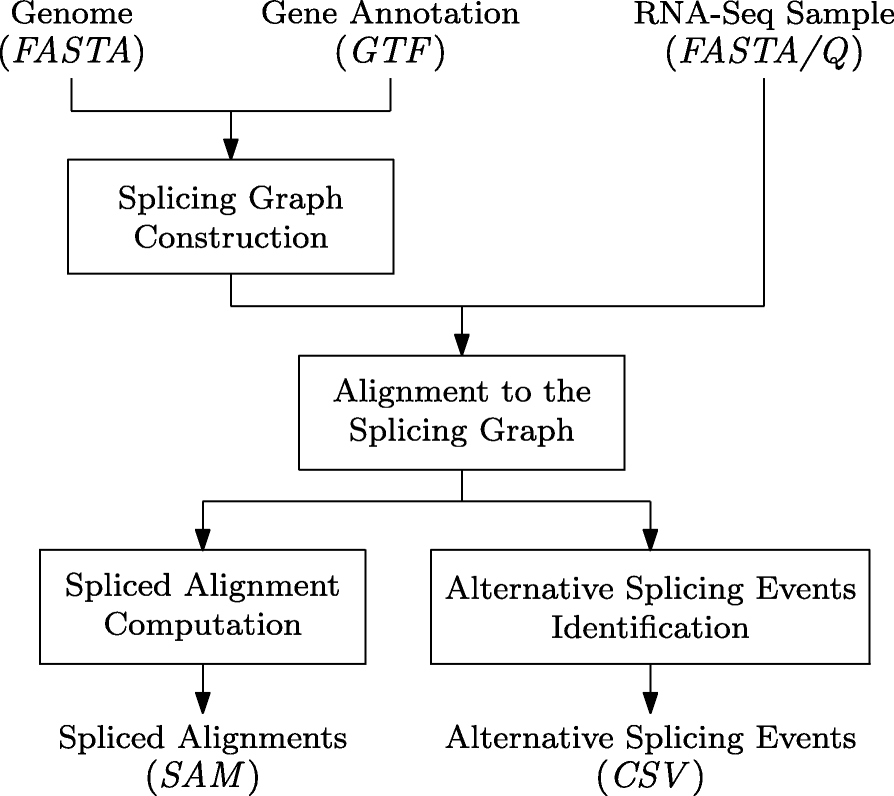
\includegraphics[width=\textwidth]{images/asgal.png}
  \caption{Il funzionamento di ASGAL illustrato}
  \label{fig:ASGAL}
\end{figure}

    	\subsection{Alternative Splicing}

L'alternative splicing è un meccanismo utilizzato dalle cellule per produrre proteine (o per meglio dire, \textit{isoforme proteiche}) diverse dallo stesso gene che viene utilizzato da oltre il 75\% dei geni umani \cite{ASExon}. Diversi studi (come \cite{ASDiseases} e \cite{ASAlzheimer}) dimostrano come l'alternative splicing giochi un ruolo fondamentale nello sviluppo di diverse malattie, come ad esempio il cancro o la sindrome di Alzheimer.

Considerando un generico frammento di DNA, esso può essere diviso in esoni (parti codificanti) e introni (parti non codificanti). Durante la fase di Trascrizione gli introni vengono rimossi e la Timina viene trasformata in Uracile, ottenendo pre-mRNA. A questo punto, in un normale processo di Splicing, tutti gli esoni vengono utilizzati, nell'ordine in cui appaiono nel pre-RNA, per ottenere una proteina.

\begin{figure}[h!]
	\centering
	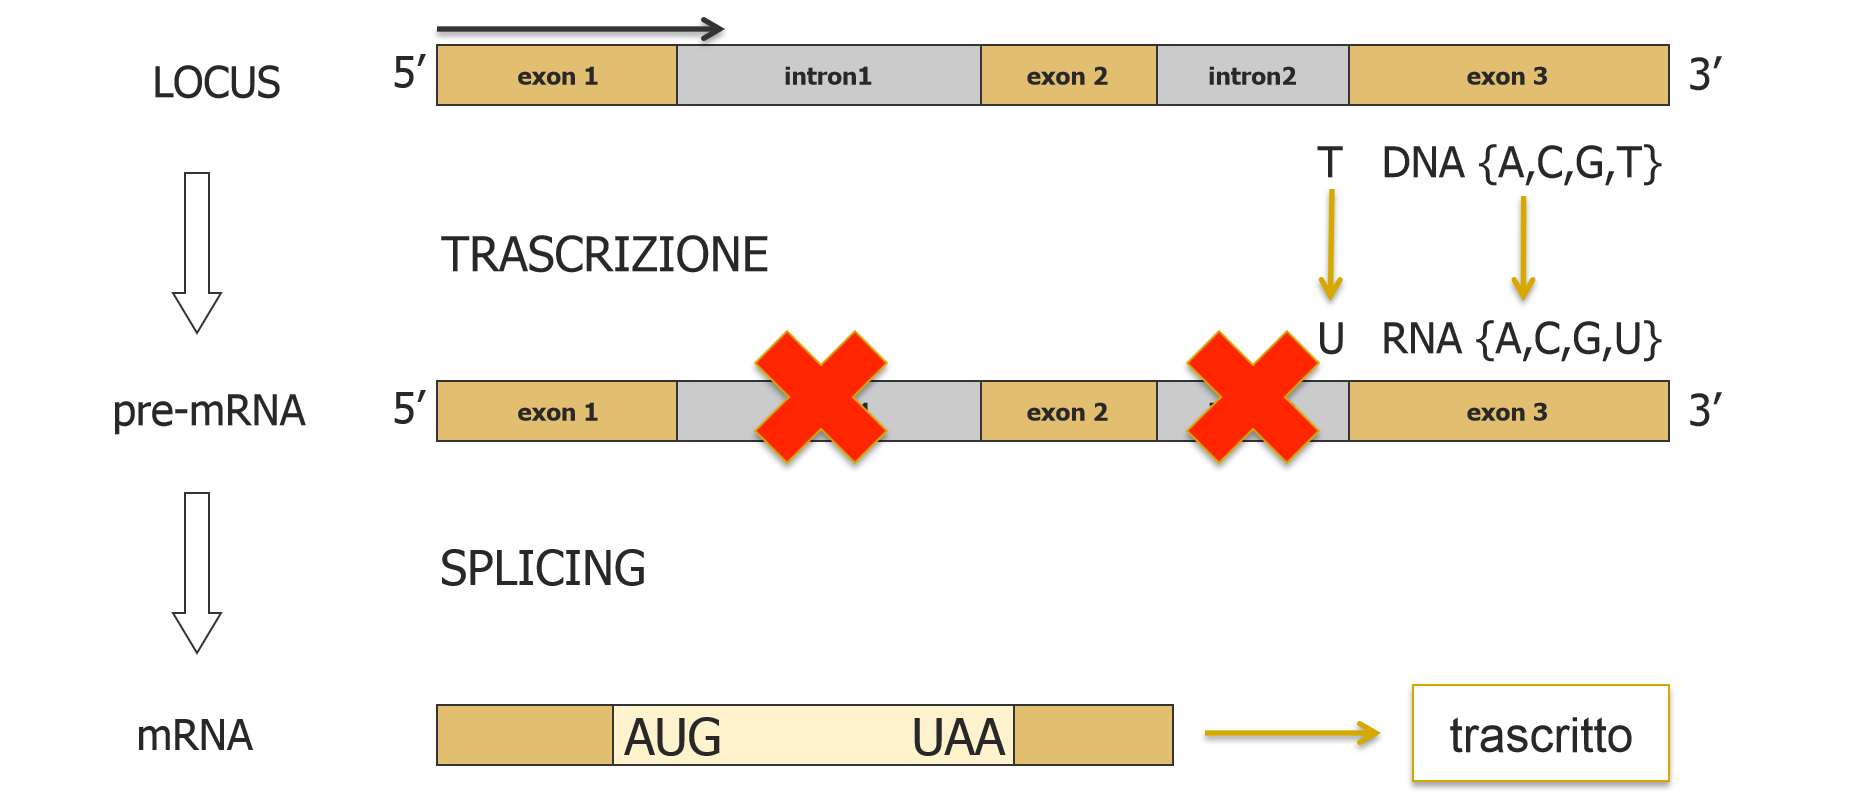
\includegraphics[width=\linewidth]{images/splicing.png}
  \caption{Trascrizione e Splicing}
  \label{fig:Splicing}
\end{figure}

Nel caso di un evento di Alternative Splicing, questo non accade: alcuni esoni potrebbero infatti non essere utilizzati, o apparire in un ordine diverso. Vengono riconosciuti 5 tipi di eventi di Alternative Splicing:

\begin{enumerate}
	\item \textbf{Exon Skipping}: Almeno un esone non appare nel trascritto
	\item \textbf{Mutually Exclusive Exons}: Almeno due esoni non compaiono mai in uno stesso trascritto
	\item \textbf{Alternative 5' Donor Site}: Parte di un introne nel 5' diventa un esone
	\item \textbf{Alternative 3' Acceptor Site}: Parte di un introne nel 3' diventa un esone
	\item \textbf{Intron Retention}: Parte di un esone diventa un introne
\end{enumerate}

ASGAL è in grado di rilevarli tutti tranne il caso 2.

\newpage

\begin{figure}[t!]
	\centering
	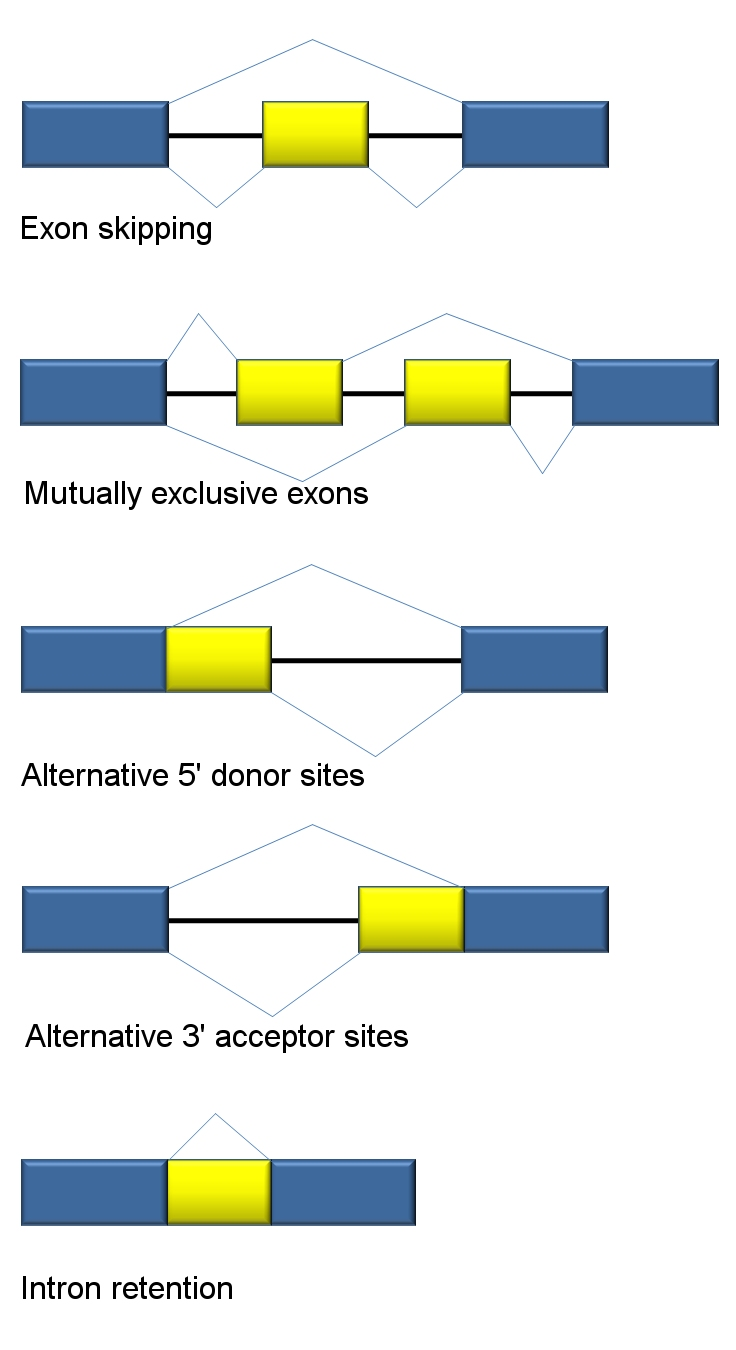
\includegraphics[height=10cm,width=10cm]{images/alternativesplicingevents.jpg}
  \caption{I diversi tipi di Alternative Splicing}
  \label{fig:AlternativeSplicingTypes}
\end{figure}

\subsection{Paired-End Reads}
Le paired-end reads consistono nell'estrazione di due letture da un singolo frammento di DNA, contrariamente alle single-end reads che ne estraggono solo una. Sono prodotte da sistemi NGS, e la loro preparazione è molto semplice: una volta stabilita la grandezza della singola lettura, viene estratta la lettura sull'estremità sinistra, il campione viene girato, e viene estratta nuovamente l'estremità sinistra (ottenendo quindi l'estremità destra). 

Viene inoltre fornita la distanza tra le due letture.

\begin{figure}[h!]
	\centering
	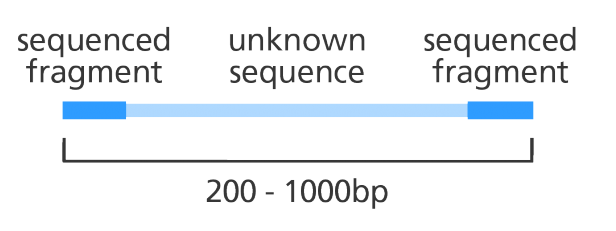
\includegraphics{images/pairedendreads2.png}
  \caption{Read paired-end}
  \label{fig:PairedEndReads}
\end{figure}
    	%\subsection{Paired-End Reads}
Le paired-end reads consistono nell'estrazione di due letture da un singolo frammento di DNA (generalmente le due estremità), contrariamente alle single-end reads che ne estraggono solo una. Sono prodotte da sistemi NGS, e la loro preparazione è molto semplice: una volta stabilita la grandezza della singola lettura, viene estratta la lettura sull'estremità sinistra, il campione viene girato, e viene estratta nuovamente l'estremità sinistra (ottenendo quindi l'estremità destra). Viene inoltre fornita la distanza tra le due letture, che permette di disambiguare alcuni casi di allineamento.

%RNA-Seq?

\begin{figure}[b!]
	\centering
	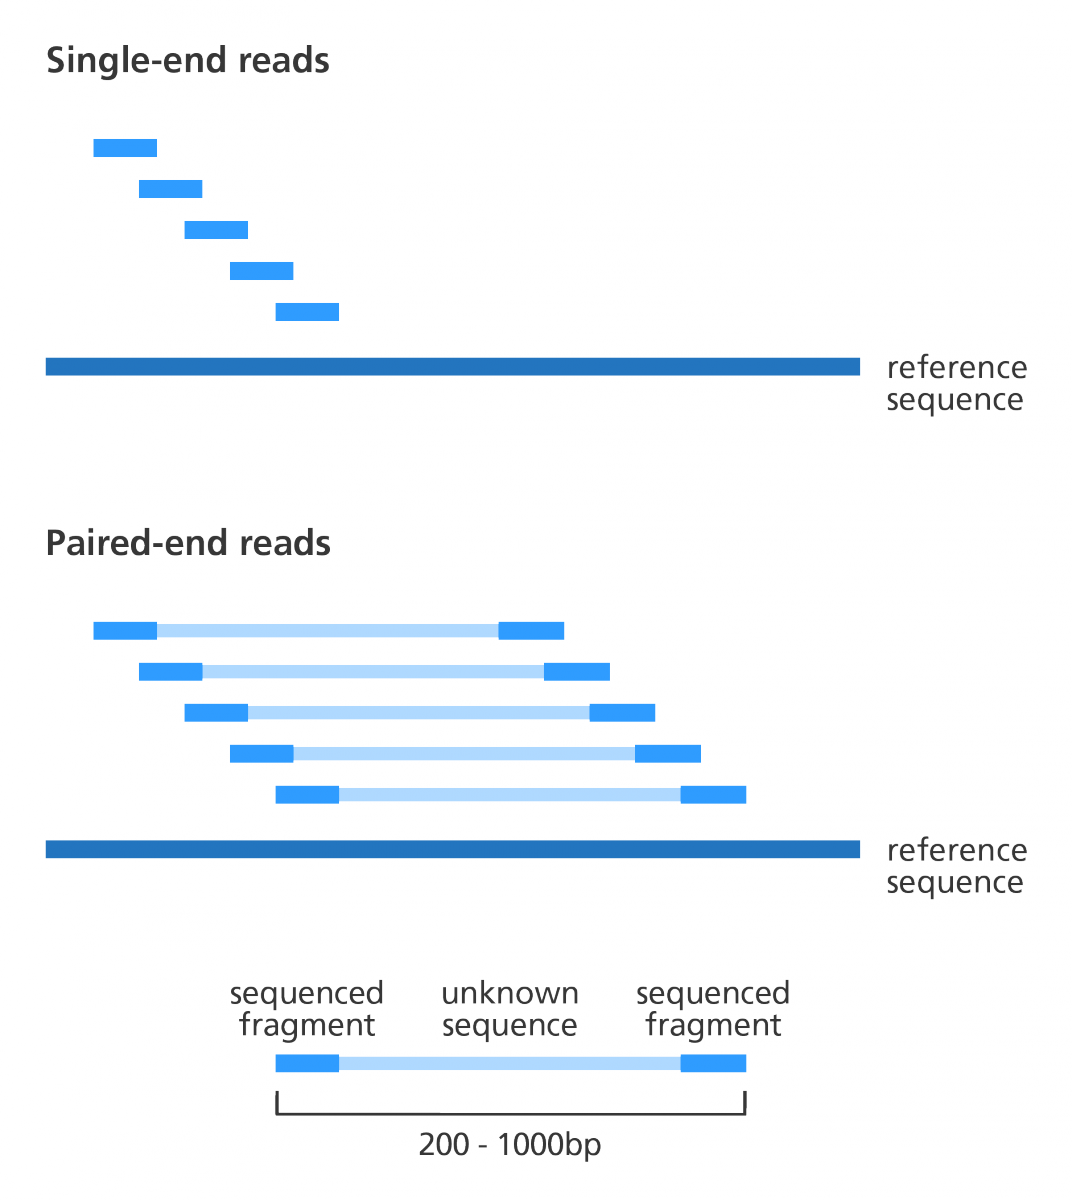
\includegraphics[height=15cm,width=10cm]{images/pairedendreads.png}
  \caption{Esempi di read single-end e paired-end}
  \label{fig:AlternativeSplicingTypes}
\end{figure}
    	
%    \section{Modifiche effettuate ad ASGAL}
    	  
    	\section{Generazione dello Splicing Graph e allineamento Splice-Aware}

\subsection{Descrizione generale}

Il primo compito di ASGAL è quello di generare lo Splicing Graph a partire dal genoma di riferimento (in formato FASTA\footnote{\url{https://blast.ncbi.nlm.nih.gov/Blast.cgi?CMD=Web&PAGE_TYPE=BlastDocs&DOC_TYPE=BlastHelp}}) e dalla sua annotazione (in formato GTF\footnote{\url{https://www.ensembl.org/info/website/upload/gff.html}}). Uno splicing graph è un grafo orientato in cui i nodi rappresentano gli esoni, e gli archi collegano due esoni che compaiono uno dopo l'altro in un trascritto; utilizzando la chiusura transitiva ogni esone viene poi collegato a tutti i suoi successori.

Per permettere un allineamento tra due stringhe viene generata una linearizzazione dello Splicing Graph, ottenuta semplicemente concatenandone i nodi e utilizzando un carattere speciale come delimitatore tra un nodo e un altro. 

Questa prima fase non utilizza le read paired-end, e non è stata quindi modificata nell'adattamento al nuovo tipo di read.

\begin{figure}[h!]
	\centering
	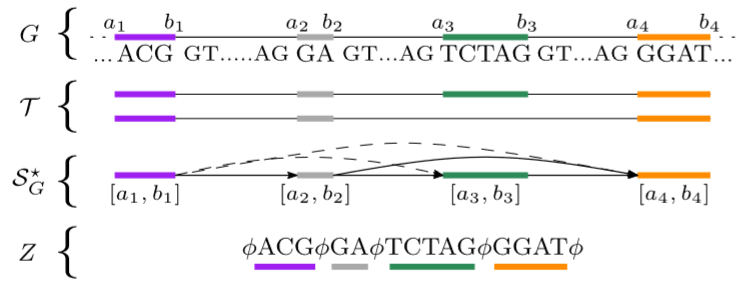
\includegraphics{images/splicinggraph.png}
  \caption{Un esempio di Splicing Graph}
  \label{fig:PairedEndReads}
\end{figure}

Il secondo compito di ASGAL è quello di allineare le read paired-end con la linearizzazione appena ottenuta. Per fare questo, utilizza il concetto di MEM (Maximum Exact Matches), ovvero di una tripla così costituita:
\begin{enumerate}
	\item Posizione iniziale nel genoma
	\item Posizione iniziale nella read
	\item Lunghezza della parte in comune
\end{enumerate}
	
Come si può intuire dal nome, i MEM utilizzano il concetto di pattern matching esatto, rispetto  ai generici algoritmi di allineamento che ammettono dei mismatch o degli indel; ad ogni allineamento corrispondono uno o più MEM.

Il nuovo formato paired-end è stato qui utilizzato per velocizzare il processo di allineamento ove possibile. Al momento non sono state utilizzate per migliorare l'efficacia dell'allineamento; si rimanda alla sezione "Sviluppi futuri" per informazioni su come questo potrebbe accadere.

\newpage

Il risultato dell'allineamento sarà restituito, per comodità, nel formato \textit{.mem}\footnote{MEM indica in generale i Maximum Exact Matches, \textit{.mem} o \textit{mem} indica il formato di file che contiene tutti i MEM generati a partire da un file contente una o più read} così composto:

\begin{itemize}
	\item Lo \textbf{strand} dell'allineamento
	\item	Il \textbf{nome della read} allineata
	\item Il \textbf{numero di errori} commessi nell'allineamento 
	\item Il \textbf{MEM} vero e proprio, eventualmente anche più di uno
	\item La \textbf{sottostringa della read} che costituisce il MEM considerato
\end{itemize}

\subsection{Allineamento di entrambe le read}
%Il primo problema da affrontare è ovviamente il fatto che sia ora necessario allineare due read per ciclo e non una; fortunatamente si tratta solo di iterare il processo di allineamento su una coppia di read ad ogni ciclo, anziché su read singola. Verranno quindi generati due file contenti MEM anziché uno. Sarà poi compito della Formattazione SAM "fondere" i due file MEM per ottenere un SAM Completo.
La prima differenza sostanziale rispetto al caso single-end è che nel caso paired-end le read da allineare sono sostanzialmente due (ovvero le due estremità); bisogna inoltre tenere conto della distanza tra di esse. 

Mentre in un generico allineatore questo avrebbe creato non pochi problemi, in ASGAL la soluzione è banale: basta trattare le due estremità come read singole, e allinearle indipendentemente. Questo è possibile in quanto ciò che si vuole ottenere è un insieme di MEM, e non siamo interessati all'ottimizzazione globale dell'allineamento. %Rivedere?

Resta comunque fondamentale riuscire a collegare i MEM delle due estremità tra di loro. Per fare questo, abbiamo deciso di utilizzare due file .mem anziché uno, con la seguente proprietà: una stessa riga nel primo file e nel secondo corrispondono alla stessa read. Questo risolve il problema del collegamento tra MEM provenienti dalla stessa read, e indirettamente anche quello della distanza tra le estremità (dati i MEM è possibile calcolare la distanza).

Non è però detto che entrambe le estremità siano coinvolte nello stesso numero di allineamenti (potrebbero addirittura non esserlo affatto). E' quindi necessario introdurre nuovi tipi di MEM per questi casi.


\subsection{Introduzione di read unmapped e placeholder nel formato mem}
Nei file mem ottenuti dallo Splice-Aware Aligner vengono ora visuallizati due nuovi tipi di MEM: quelli relativi alle read unmapped e quelli relativi ai placeholder. Il primo caso è banale, e rappresenta tutte quelle read che non hanno un matching esatto di lunghezza considerevole con il genoma dato in input.

Il secondo caso è più complesso e rappresenta un insieme di read fasulle utilizzate solo come padding per avere due file MEM della stessa lunghezza: questo facilita enormemente l'elaborazione nello step successivo. 
\newpage

Come detto in precedenza quando si lavora con read paired-end è sempre necessario lavorare a coppie, ma non sempre ad uno stesso pair è associato lo stesso numero di allineamenti secondari: è qui che entrano in gioco i placeholder. 

I placeholder sono stati implementati in questo modo: si tengono due contatori (che rappresentano rispettivamente il numero di allineamenti relativi alla prima read e quelli relativi alla seconda read), si ottengono separatamente gli allineamenti relativi a ciascuna delle due read, e si controllano i contatori. Si prende il minore dei due e si aggiungono tanti placeholder quanto bastano per rendere uguali i contatori.

Il seguente frammento di codice mostra la procedura:

\begin{lstlisting}[language=C++]
        //head_1 and head_2 are the IDs of the alignments
        if (count1 < count2) {
            while (count1 < count2) {
                outFile_1 << "PLACEHOLDER" << " " << head_1 << "\n";
                count1++;
            }
        } else if (count2 < count1) {
            while (count2 < count1) {
                 outFile_2 << "PLACEHOLDER" << " " << head_2 << "\n";
                 count2++;
            }
        }
\end{lstlisting}


E' stato inoltre necessario introdurre un nuovo campo nel formato \textit{.mem}, che permette di distinguere il tipo di MEM preso in esame: ad esempio trovando come primo valore la stringa "MAPPED", si capisce che il MEM preso in esame è relativo ad una read che è stata mappata correttamente; ovviamente vale lo stesso ragionamento con le stringhe "UNMAPPED" e "PLACEHOLDER".

L'immagine seguente mostra un esempio di file nel nuovo formato mem:

\begin{figure}[h!]
	\centering
	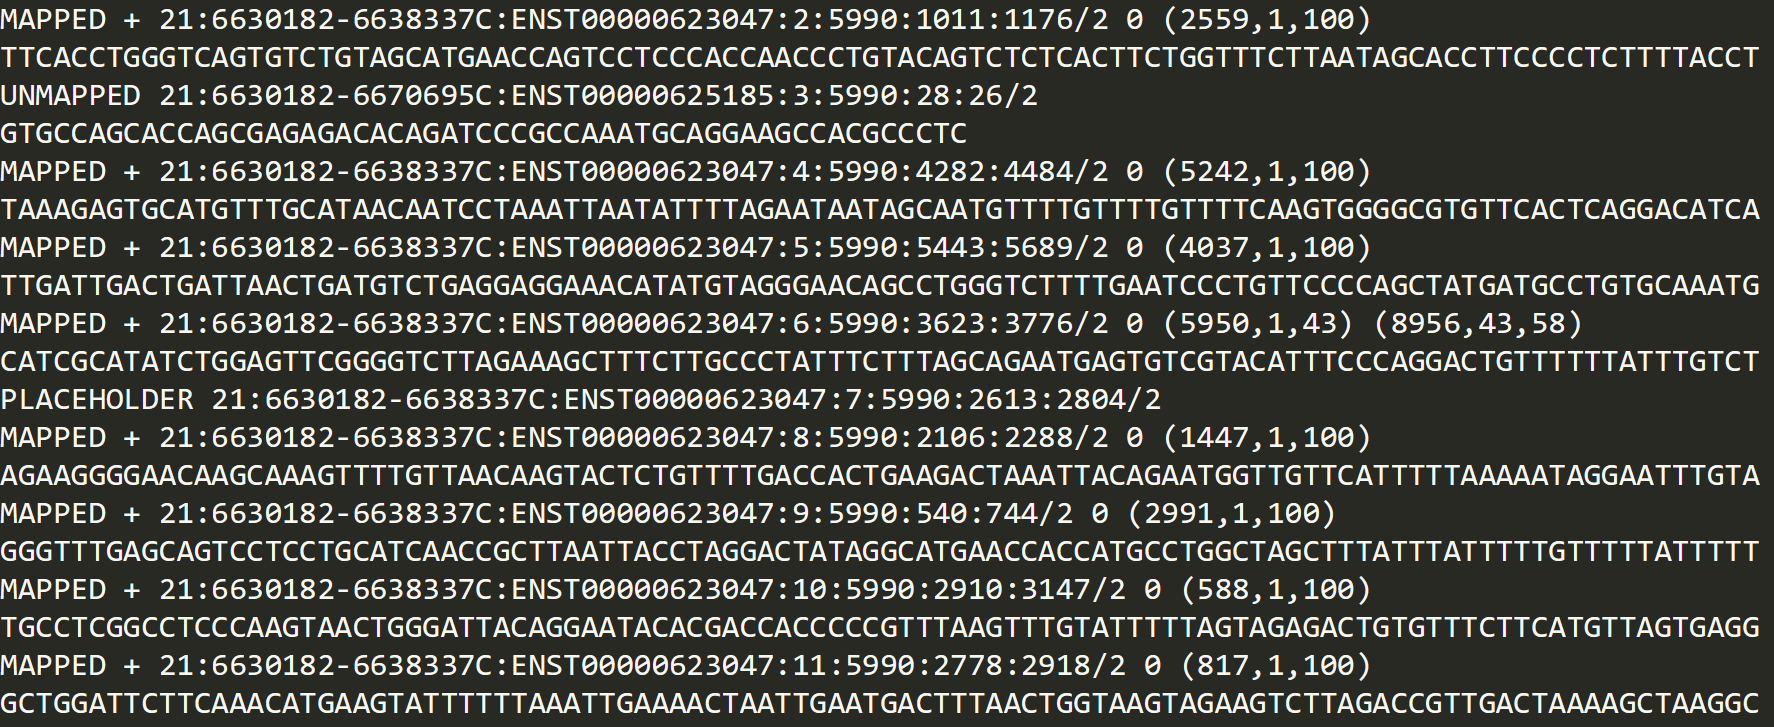
\includegraphics[width=\linewidth]{images/tipiMEM4.png}
  \caption{Esempio di file in formato \textit{.mem}}
  \label{fig:MEMTypes}
\end{figure}

\newpage

\subsection{Supporto alle fragment library types}
Ci sono diversi protocolli per la preparazione di librerie paired-end, che portano a read con caratteristiche diverse. Le \textbf{fragment library types}\footnote{\url{https://salmon.readthedocs.io/en/latest/}} permettono di descrivere queste caratteristiche in modo sintetico. Le caratteristiche che possono essere descritte sono:
\begin{itemize}
	\item \textbf{Orientamento relativo di una read rispetto all'altra}: può essere inward (I) o outward (O)
	\item \textbf{Se è noto o meno lo strand di appartenenza delle due read}:  può essere stranded (S) o unstranded (U)
	\item \textbf{La direzionalità della prima read, solo nel caso stranded}: può essere first (F) o reverse (R)
\end{itemize}

La seguente immagine descrive tutte le possibili combinazioni:
\begin{figure}[h!]
	\centering
	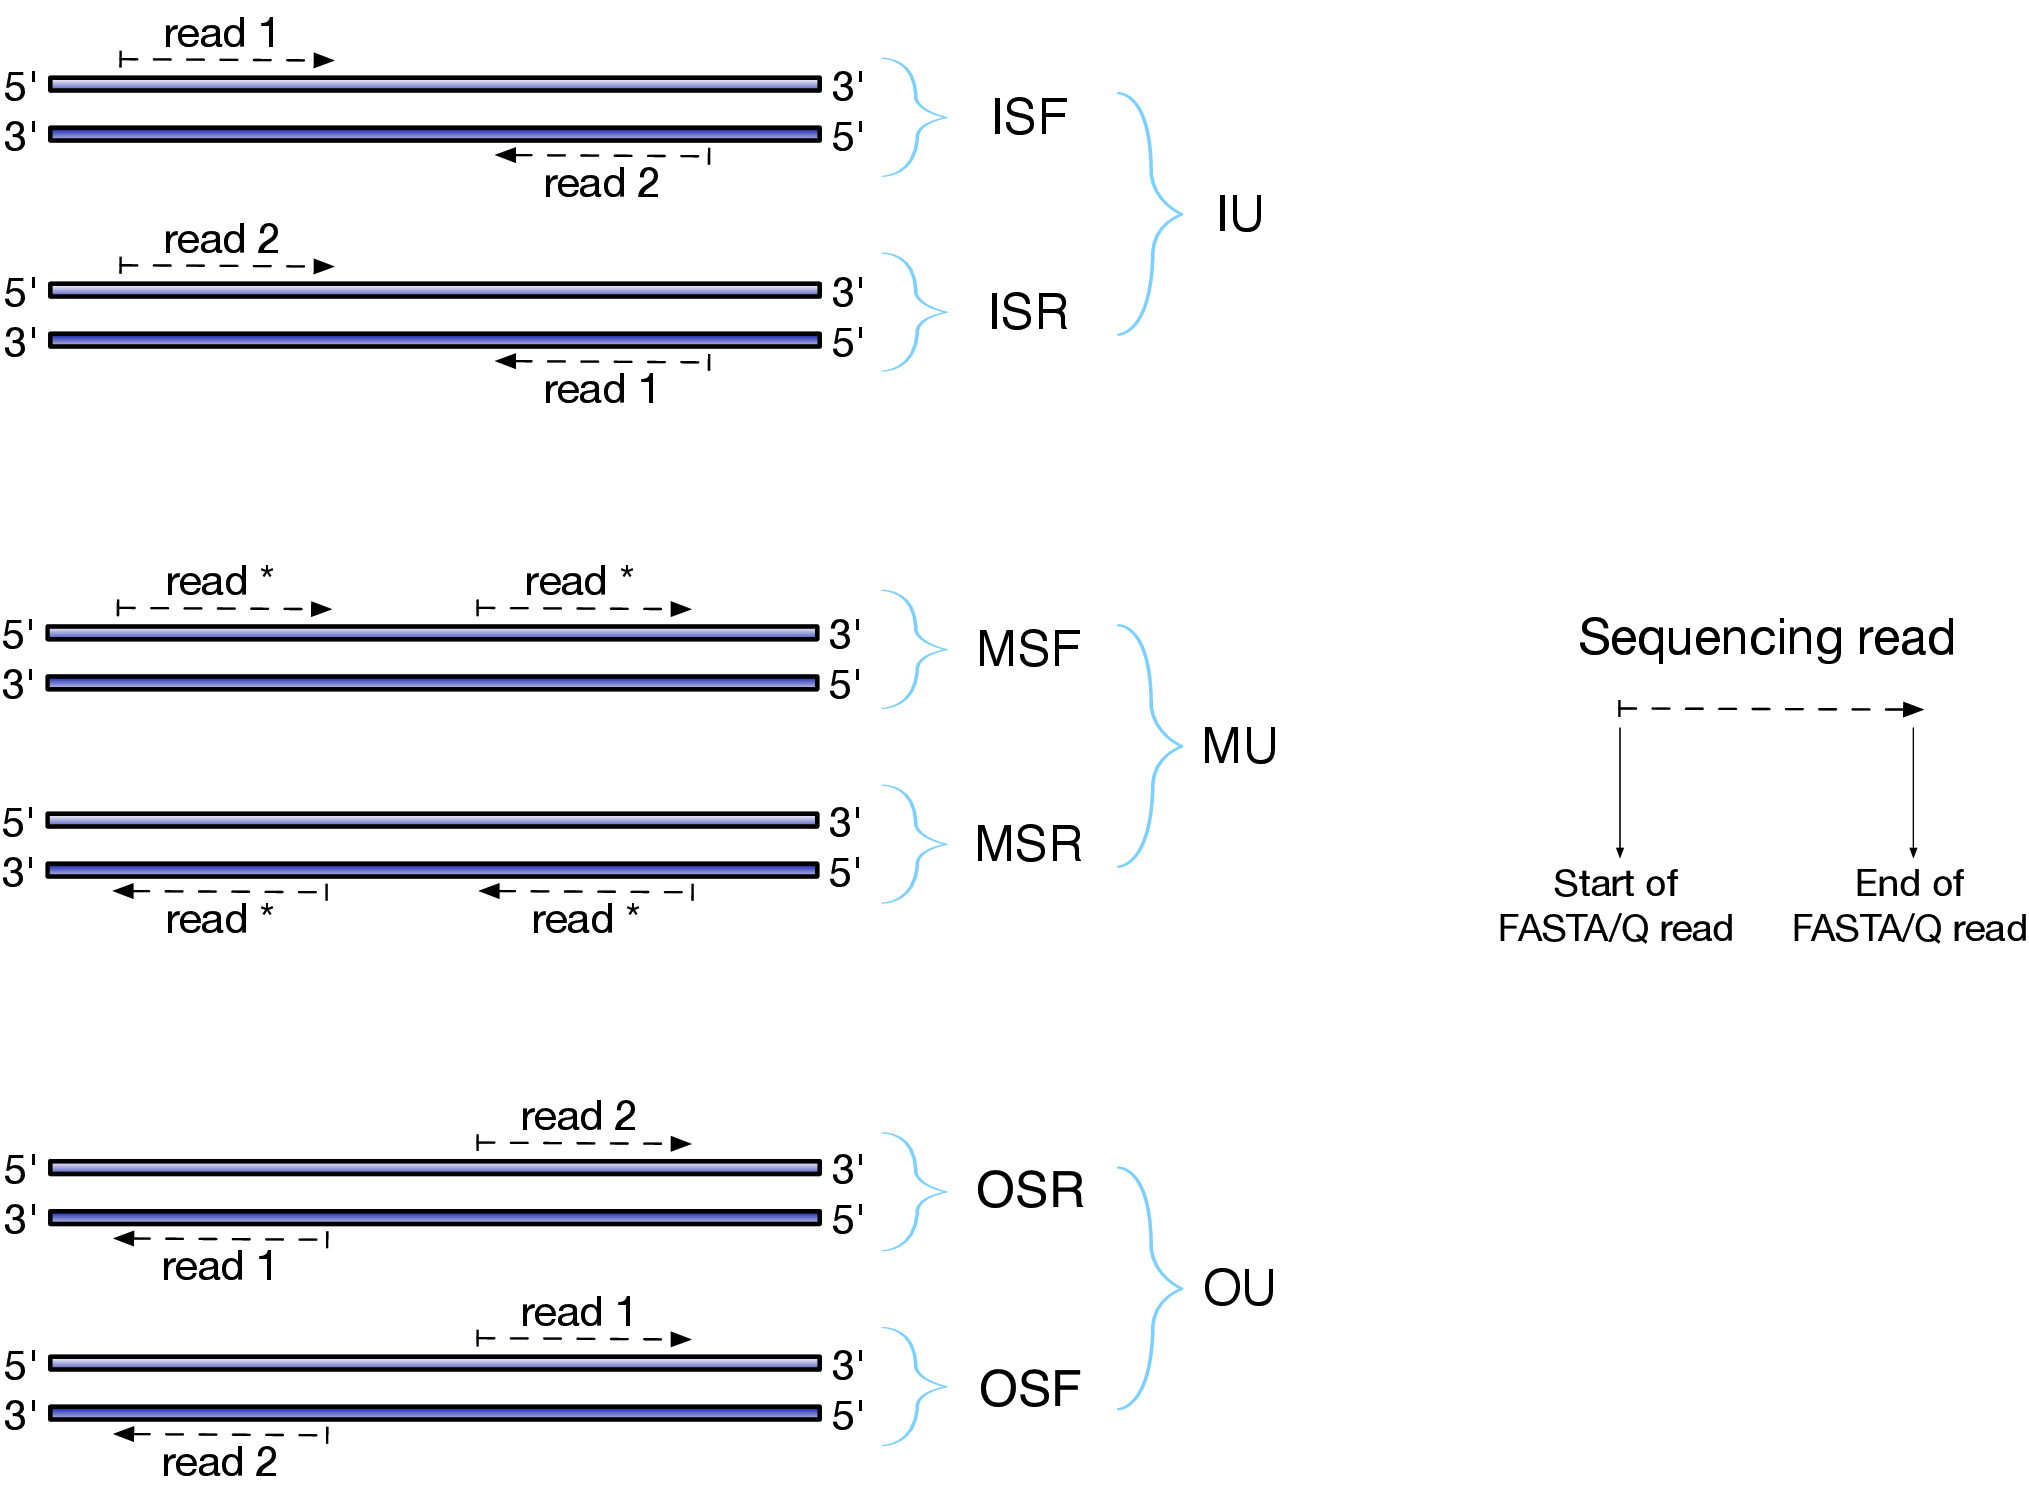
\includegraphics[width=\linewidth, height=10cm]{images/fragmentlibrarytypes.png}
  \caption{I diversi tipi di fragment library types}
  \label{fig:FragmentLibraryTypes}
\end{figure}

\newpage

ASGAL utilizza queste informazioni per velocizzare il processo di allineamento. Nel formato single-end questa informazioni non esiste, quindi ogni read veniva allineata in entrambe le direzioni, e si prendeva l'allineamento migliore dei due. 

Nel formato paired-end, si può utilizzare la ftl per ridurre il numero di allineamenti necessari, fino al 50\% nel caso stranded. Ad esempio, se viene fornita un ftl di tipo ISF è sufficiente allineare la read 1 sullo strand + (ignorando lo strand -) e la read 2 sullo strand - (ignorando lo strand +).

Il caso unstranded richiede un po' più di attenzione: non è infatti possibile sapere a priori su quale strand allineare la prima read. Per risolvere questo problema è stata riutilizzata la vecchia procedura di allineamento della prima read in entrambe le direzioni; una volta trovata la direzione migliore per la prima, la seconda viene di conseguenza. 

Supponiamo ad esempio di avere una libreria in formato MU: se la prima read allinea sullo strand +, di conseguenza anche la seconda sarà allineata sullo strand +; viceversa, se la prima read allinea sullo strand -, anche la seconda allinea sempre sullo strand -. In questo caso si ottiene solo una riduzione del 25\% nel numero degli allineamenti.

Qualora il tipo di libreria non venga fornito dall'utente, rimane necessario provare ad allineare le read in entrambe le direzioni, senza alcun incremento di prestazioni.



    	\section{Conversione in formato SAM}

\subsection{Cos'è e come funziona}
Come già detto, gli allineamenti ottenuti dallo Splice-Aware aligner sono in un formato non standard chiamato MEM (nota: l'acronimo MEM si riferisce sia al formato dell'output che all'estensione del file ottenuto). L'obiettivo di questa seconda parte è quello di convertire i due file MEM in un singolo file SAM (Sequence Alignment Map), il formato standard per memorizzare gli allineamenti.

Non si tratta solo di una semplice conversione, in quanto è necessario indurre diverse informazioni aggiuntive per avere un file SAM standard, quali: la posizione di inizio dell'allineamento sulla genomica, la stringa CIGAR, i flag relativi all'allineamento, ecc. Per supportare le read paired-end è stato necessario modificare gran parte di queste funzionalità.

In questa sezione saranno descritte le principali modifiche apportate al Formattatore SAM, oltre ad alcune funzionalità aggiuntive utili per la rilevazione di eventi di Alternative Splicing.

\newpage

\subsection{Formato SAM}
Il formato SAM (Sequence Alignment Map) è composto da 11 campi:

\begin{enumerate}
	\item QNAME: Il nome identificativo dell'allineamento
	\item FLAG: Una serie di flag binari che identificano le caratteristiche dell'allineamento
	\item RNAME: Identificativo del gene di riferimento
	\item POS: Posizione 1-based di inizio dell'allineamento sul genoma
	\item MAPQ:  Qualità dell'allineamento
	\item CIGAR: Stringa che identifica le operazioni effettuate per ottenere l'allineamento
	\item RNEXT: QNAME del mate (solo paired-end)
	\item PNEXT: POS del mate	(solo paired-end)
	\item TLEN:  Distanza tra mate (solo paired-end)
	\item SEQ:  	Allineamento vero e proprio
	\item QUAL: Valore Phread della read
\end{enumerate}

\begin{figure}[h]
	\centering
	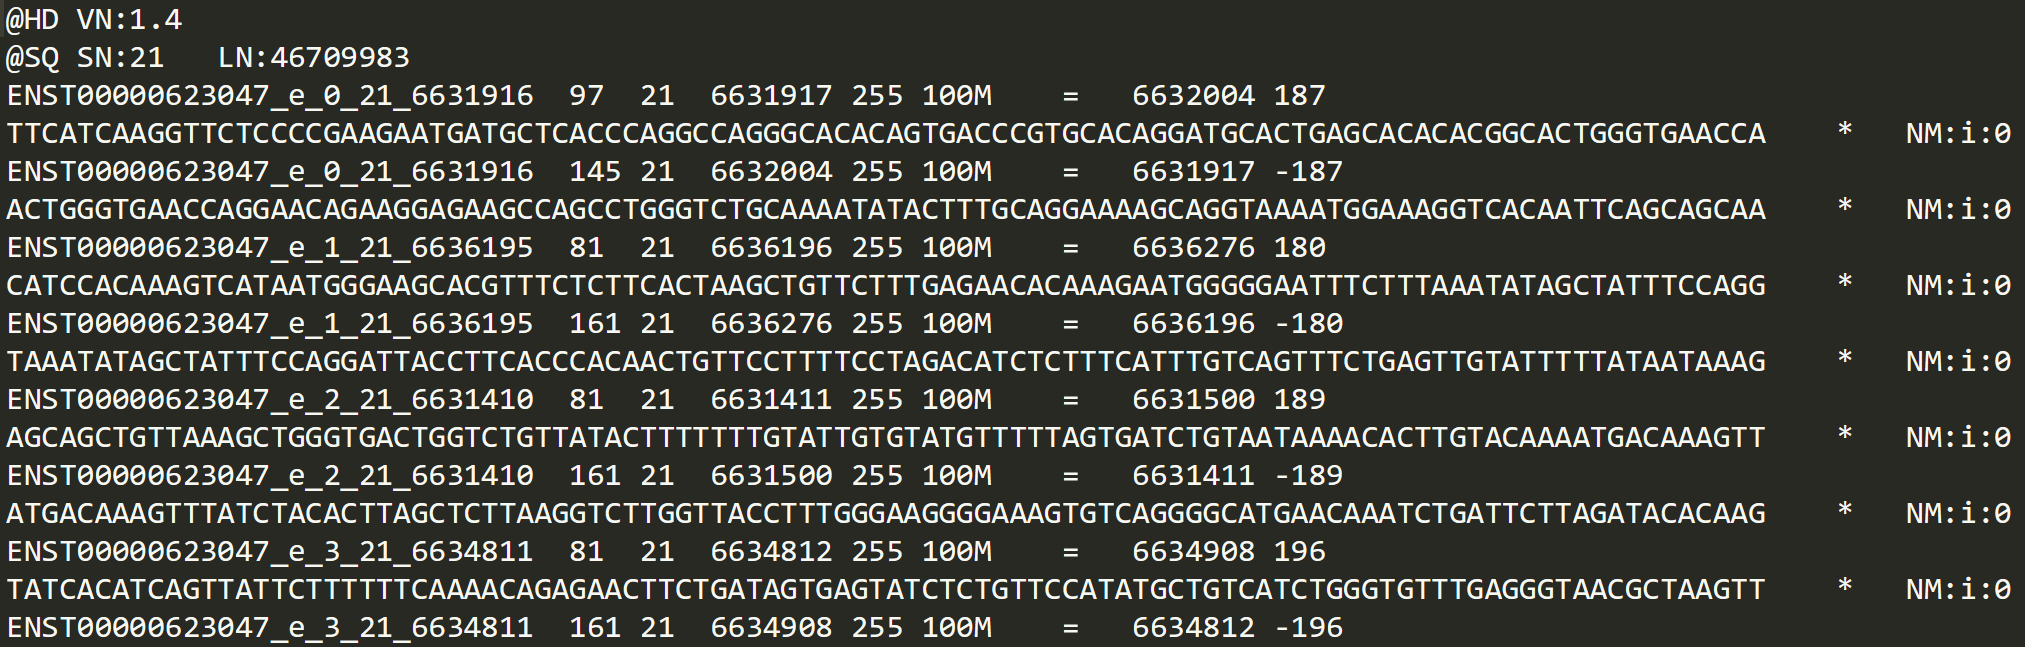
\includegraphics[width=\linewidth]{images/esempioSAM.png}
  \caption{Un esempio di file SAM prodotto da ASGAL}
  \label{fig:AlternativeSplicingTypes}
\end{figure}

\newpage

\subsection{Modifiche alla computazione del campo FLAG}
Il campo FLAG è il secondo del formato SAM e consiste di un valore numerico (ottenuto convertendo in decimale una serie di flag binari) che rappresenta le caratteristiche dell'allineamento preso in esame. La seguente immagine mostra il significato di ciascun bit del flag:

\begin{figure}[h]
	\centering
	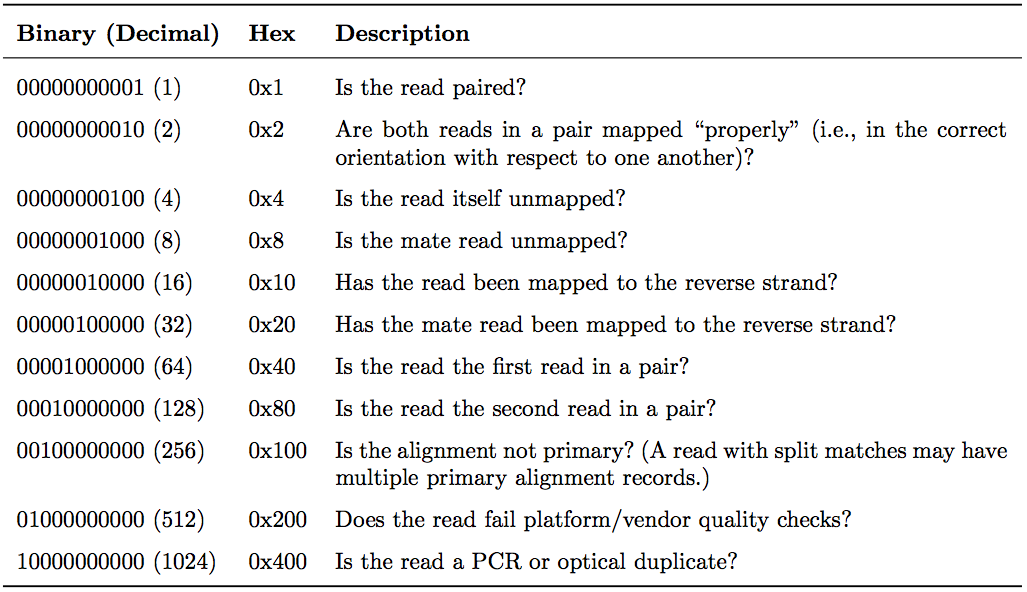
\includegraphics[width=\linewidth]{images/samflag.png}
  \caption{Il significato di ciascun bit del campo FLAG }
  \label{fig:SAM Flags}
\end{figure}

Nei casi single-end solo due flag vengono utilizzati: quello relativo allo strand (0x16) e quello relativo al tipo di allineamento (0x100); visto che le read non sono paired, il flag 0x1 sarà sempre false, quindi tutti i flag risultanti saranno pari.

Nei casi paired-end tutti i flag vengono utilizzati. E' inoltre necessario trattare gli allineamenti a coppie, in quanto il campo FLAG esprime informazioni anche sul mate e non solo sull'allineamento preso in esame. 

Supponiamo ad esempio di avere due read, la prima che mappa sullo strand positivo e la seconda che non mappa (ed è quindi \textit{unmapped}). Sarà innanzitutto necessario mettere a true il flag relativo alle read paired-end (0x1) per entrambe le read. Considerando la prima, sarà messo a true il flag relativo al mate unmapped (0x8) e il flag relativo al first-in-pair (0x4). Considerando la seconda, sarà messo a true il flag relativo alla read unmapped (0x4) e quello relativo al second-in-pair(0x80). I flag in decimale saranno quindi 73 e 133.

Si noti che per il momento non viene tenuto conto dei flag 0x200 e 0x400, ma questo non è di alcuna rilevanza al fine di identificare eventi di Alternative Splicing.

\newpage

\subsection{Calcolo dei campi RNEXT, PNEXT e TLEN}
I campi TLEN, RNEXT e PNEXT rappresentano rispettivamente il settimo, l'ottavo e il nono campo di ogni record del formato SAM; essi sono praticamente inutilizzati quando si allineano read single-end, ma nel formato paired-end assumono maggiore importanza. In particolare i campi RNEXT e PNEXT sono utilizzati da strumenti di visualizzazione degli allineamenti (come ad esempio IGV) per permettere una corretta visualizzazione di una read e del suo mate.

Il campo RNEXT contiene il nome dell'allineamento relativo al mate (ovvero il suo campo PNAME). Per semplicità, quando i due allineamenti sono consecutivi, si può lasciare il suo valore a '='.

Il campo PNEXT contiene la posizione iniziale 1-based dell'allineamento relativo al mate (ovvero il suo campo POS. Qualora il mate fosse unmapped, si utilizza il valore 0.

Il campo TLEN rappresenta la distanza la lunghezza del template osservato, ovvero la distanza (sul genoma) tra l'inizio della prima read e la fine della seconda. Per la sua computazione è sufficiente trovare la posizione finale del secondo allineamento e sottrarre la posizione iniziale del primo.

La seguente immagine mostra un esempio di allineamento visualizzato da IGV:

\begin{figure}[h]
	\centering
	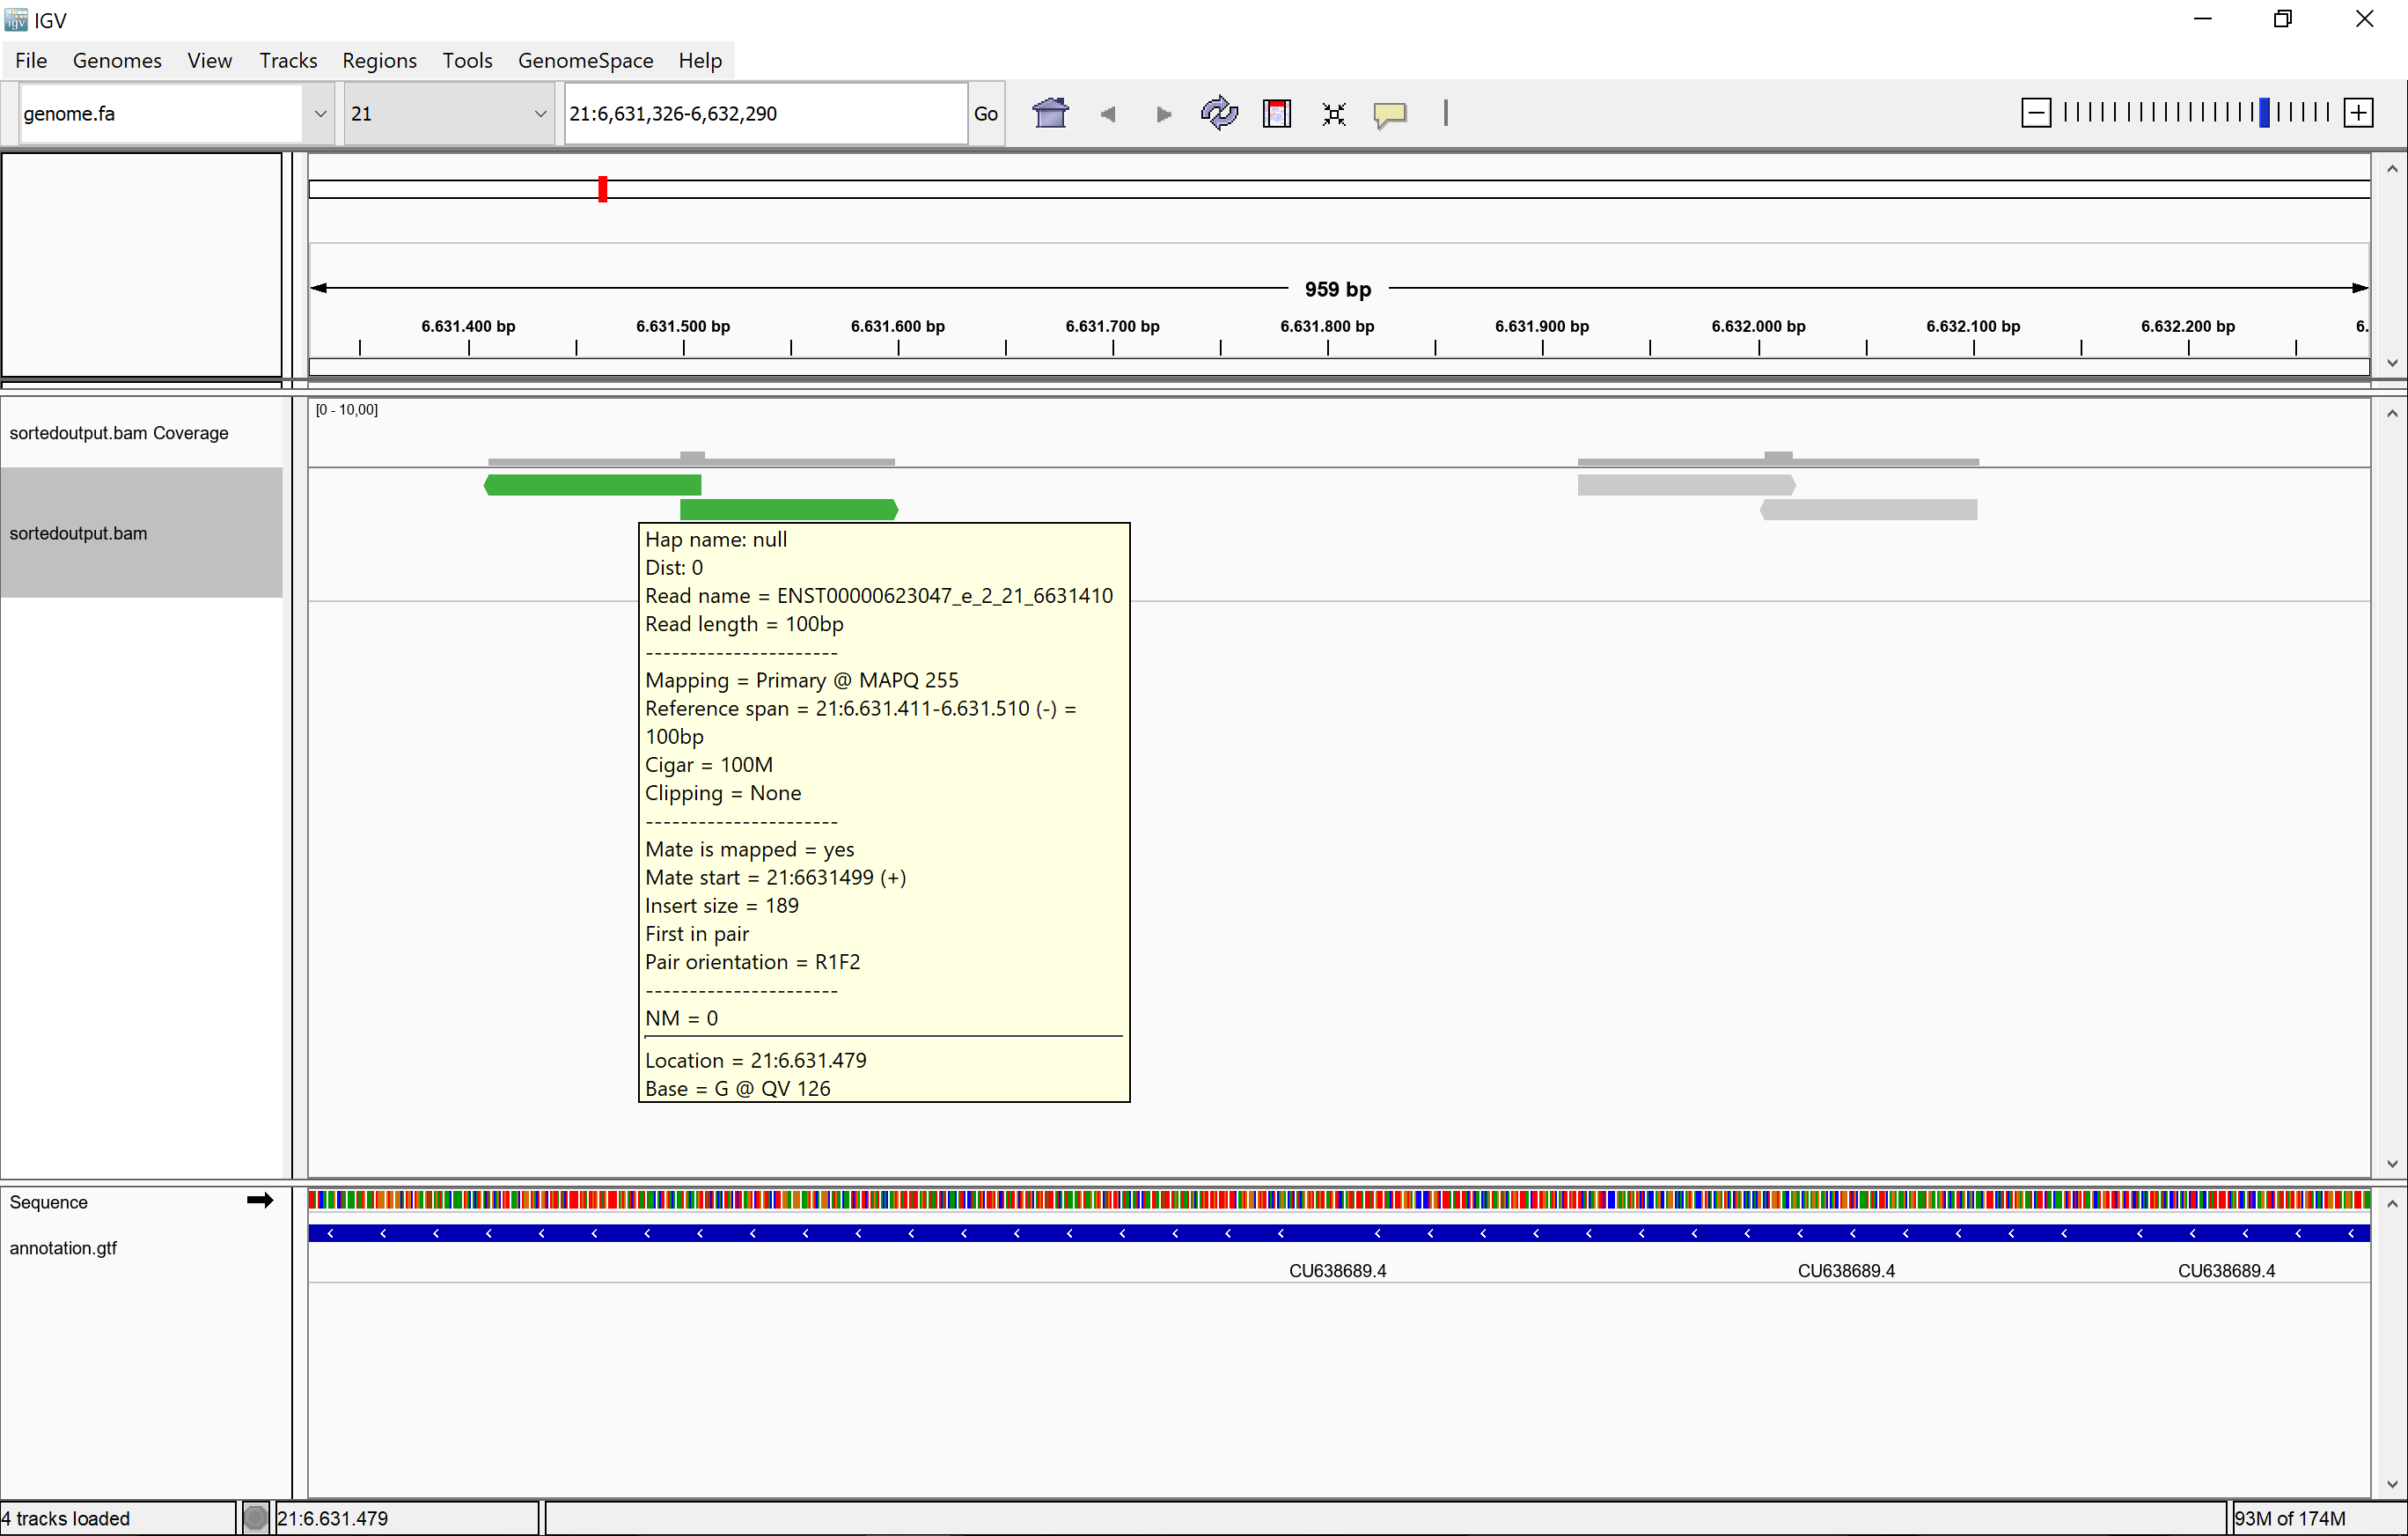
\includegraphics[width=\linewidth]{images/mateinfo.png}
  \caption{Informazioni su mate da SAM formato correttamente}
  \label{fig:Mate info}
\end{figure}

\newpage

E' importante notare che, se questi campi sono settati correttamente, lasciando il cursore del mouse su un allineamento vengono visualizzate tutte le informazioni relative al mate. Al contrario, se si prova ad indicizzare il file BAM (la versione binaria del formato SAM) per l'utilizzo con IGV, e questi campi non sono stati settati correttamente, verrà visualizzato un errore. Un esempio errore è il seguente: se il campo FLAG non contiene 0x8 (quindi il mate è mapped), e si inserisce un valore di PNEXT diverso da 0, al momento dell'indicizzazione sarà visualizzato il messaggio "mapped mate cannot have zero coordinate; treated as unmapped".

\subsection{Calcolo delle statistiche dell'allineamento}
Seguendo l'esempio di altri allineatori (come ad esempio STAR), è stato deciso di visualizzare alcune statistiche in fase di allineamento, quali:

\begin{itemize}
	\item Numero di read mappate e non mappate
	\item Numero di allineamenti primari e secondari
	\item IDMP
	\item tIDMP
\end{itemize}

Questi valori sono visualizzati nel file \textit{.alignsinfo.txt}. Anche se non hanno finalità particolari per la rilevazione di eventi di Alternative Splicing, essi forniscono uno strumento per valutare la qualità degli allineamenti effettuati da ASGAL.
\newpage
    	\section{Rilevazione degli eventi di Alternative Splicing}

\subsection{Descrizione generale}

Il Rilevatore di Eventi di Alternative Splicing si occupa di rilevare tutti gli eventi indotti dalle read. Per fare questo, confronta gli introni noti (deducibili dal file gtf) con quelli \textit{novel} (deducibili dagli allineamenti in formato mem); analizzando le differenze tra i due è possibile rilevare gli eventi di Alternative Splicing.

Trovare gli introni noti è semplice, in quanto nel file gtf sono riportati tutti gli esoni con le relative posizioni di inizio e fine: gli introni sono quindi rappresentati dalla porzione di genoma tra un esone e un altro. 

La rilevazione degli introni novel è invece più complessa, e utilizza i MEM generati dello Splice-Aware Aligner. Preso un generico allineamento, esso può essere rappresentato da uno o più MEM. Nel secondo caso viene calcolata la distanza tra di essi sia sul genoma che sul testo degli esoni; si considerano introni tutte le porzioni del genoma dove questi due valori differiscono.

\begin{figure}[h!]
	\centering
	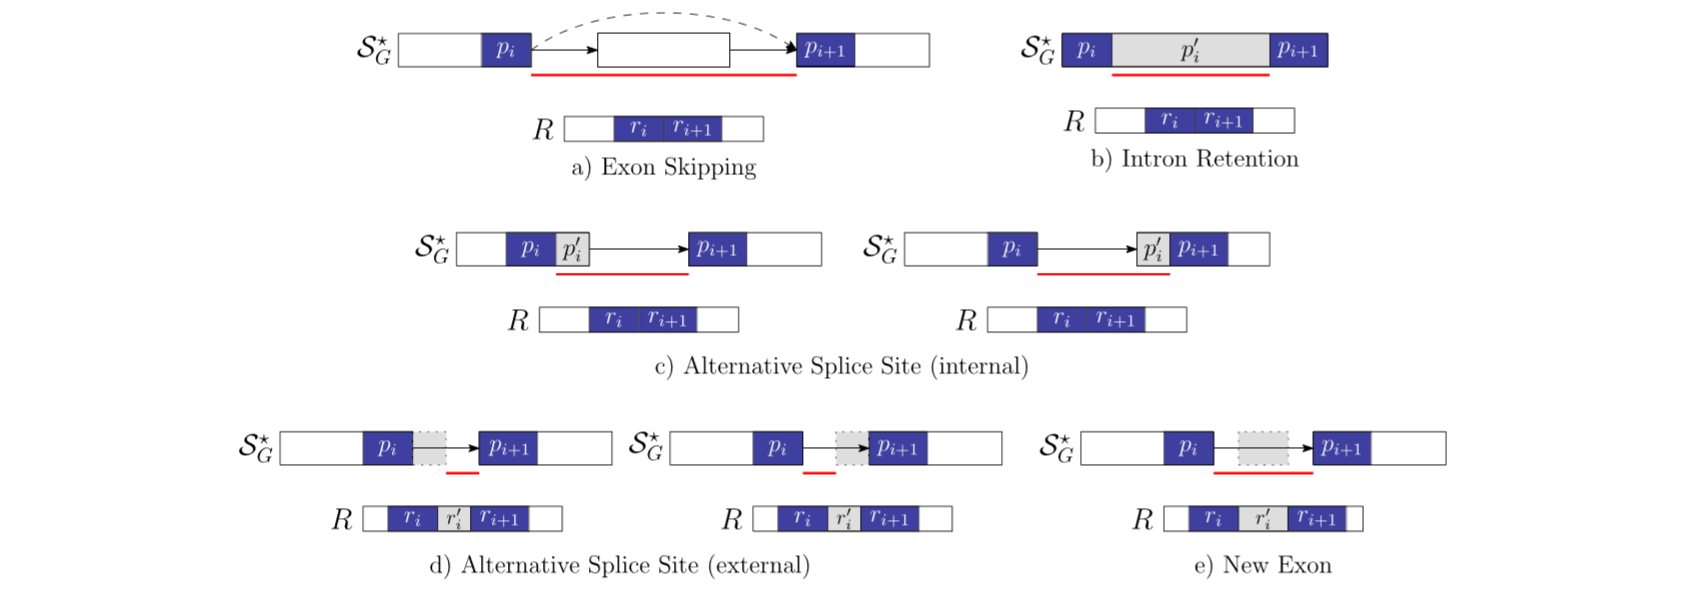
\includegraphics[width=\linewidth, height=7cm]{images/pattern.png}
  \caption{Fase di confronto degli introni}
  \label{fig:Summary1}
\end{figure}

Viene poi eseguita una fase di riconciliazione (che permette di migliorare la qualità degli introni rilevati) e vengono filtrati quelli non supportati da un numero sufficiente di read.

A questo punto avviene la procedura di rilevazione vera e propria, che confronta gli introni novel con quelli noti, utilizzando dei pattern che rappresentano i vari eventi di Alternative Splicing.

La seguente immagine riassume la procedura:

\begin{figure}[h!]
	\centering
	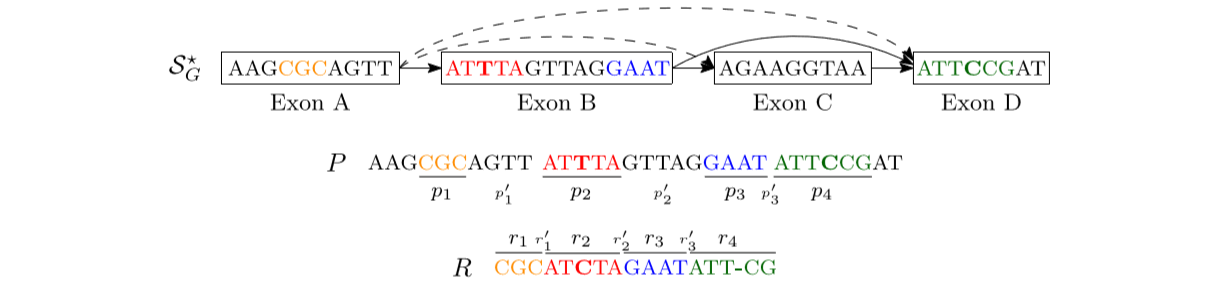
\includegraphics[width=\linewidth, height=5cm]{images/riassuntorilevazione.png}
  \caption{Riassunto della fase di rilevazione}
  \label{fig:Summary2}
\end{figure}

\newpage

Gli eventi di Alternative Splicing così rilevati saranno poi riportati in un file \textit{.events.csv}, che contiene, per ogni evento rilevato:
\begin{enumerate}
	\item Il \textbf{tipo di evento} rilevato
	\item Le \textbf{posizioni iniziali e finali} sul genoma
	\item Il \textbf{numero di read} che supportano l'evento
	\item I \textbf{trascritti} che supportano l'evento
\end{enumerate}

\subsection{Merge degli introni dedotti dai due sample}

Come già detto in precedenza, i MEM generati dallo Splice-Aware Aligner vengono utilizzati al fine di rilevare nuovi introni; ovviamente è necessario estendere questa procedura alle read paired-end. Si tratta in sostanza di fare una merge degli introni dedotti da ciascuno dei due file.

Il seguente frammento di codice mostra la procedura:

\begin{lstlisting}[language=Python]
def mergeIntrons(introns1, introns2):
    introns = {}
    for (p1,p2),w in introns1.items():
            introns[(p1,p2)] = w
    for (p1,p2),w in introns2.items():
            if (p1,p2) not in introns.keys():
                introns[(p1,p2)] = w
            else:
                introns[(p1,p2)] += w
    return introns
\end{lstlisting}

%\begin{figure}[h!]
%	\centering
%	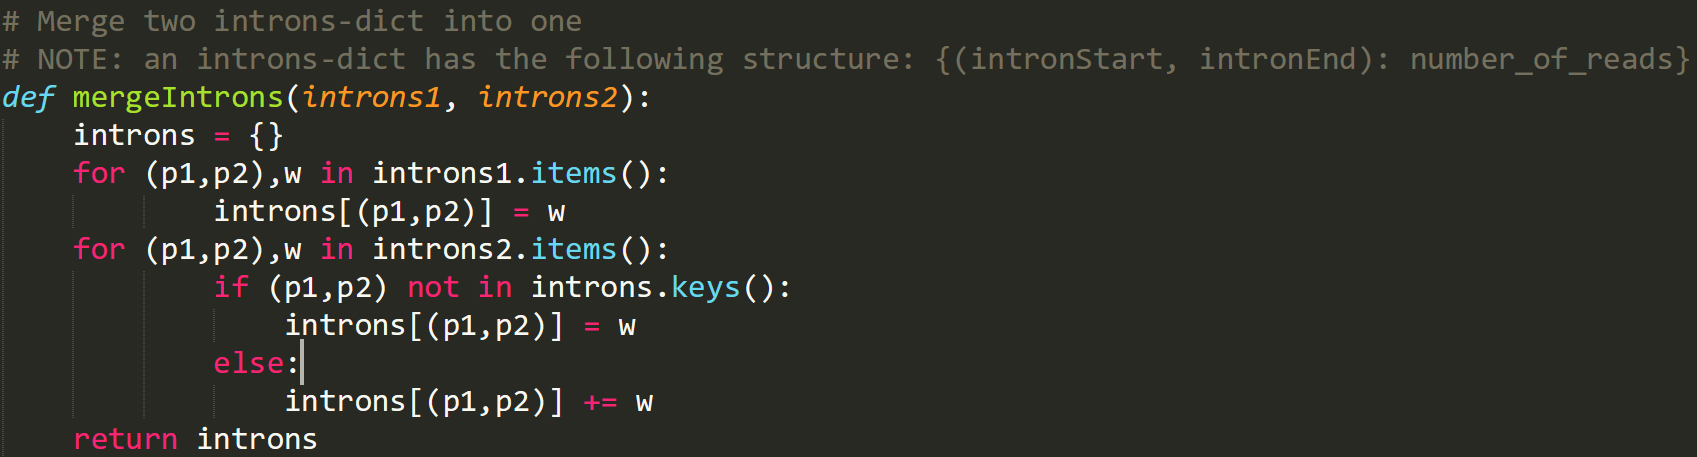
\includegraphics[width=\linewidth]{images/mergeIntrons.png}
%  \label{fig:MergeIntrons}
%\end{figure}

\newpage

\subsection{IDMP (Inner Distance between Mate Pairs)}
Considerando una coppia di read, si definisce IDMP (Inner Distance between Mate Pairs) la distanza sul genoma di riferimento tra l'ultima base della prima read e la prima della seconda. Questa informazione viene generalmente fornita dall'ente che ha effettuato il sequenziamento, e può essere confrontata con l'IDMP rilevato durante l'allineamento per rilevare nuovi eventi di Alternative Splicing.

Visto che un allineamento può essere rappresentato da più di un MEM, non è possibile semplicemente aggiungere la lunghezza dell'allineamento alla sua posizione iniziale. Prima di poter calcolare l'IDMP è quindi necessario introdurre il concetto di BitVector, ovvero una sequenza di bit che rappresenta la posizione degli esoni nello Splicing Graph. Un BitVector è dotato di due operazioni, entrambe svolte in tempo costante:

\begin{itemize}
	\item Rank: data una posizione, ritorna l'identificativo dell'esone di provenienza
	\item Select: dato un esone, ritorna la posizione di partenza 
\end{itemize}

Queste due operazioni permettono di calcolare l'IDMP in maniera efficace. Innanzitutto si prende l'ultimo MEM relativo all'allineamento della prima read, e si utilizza l'operazione di Rank per trovare l'esone di appartenenza. A questo punto, si utilizza l'operazione di Rank per trovare la posizione iniziale dell'esone. L'offset sarà quindi dato dalla differenza tra il MEM e la posizione iniziale dell'esone. Basta quindi aggiungere questo offset alla posizione iniziale per trovare la fine del primo allineamento.

% Sistemare, spiegare come viene calcolato.
L'inizio del secondo allineamento viene calcolato facendo prima la Rank sul primo MEM, e utilizzando la Select sul risultato ottenuto. A questo punto basterà sottrarre ad esso la fine di quello precedente, in modo da ottenere l'IDMP.

Il seguente frammento di codice riassume la procedura:

\begin{lstlisting}[language=Python]
def getEnd(mem, bv, exPos):
    exonN = bv.rank(mem[0])

    # get starting position (on reference)
    exonStartingPos = exPos[exonN-1][0]

    # get offset from bitvector
    exonStartingPos_onT = bv.select(exonN)
    offset = mem[0] - exonStartingPos_onT + 1;

    # find the end
    end = exonStartingPos + offset + mem[2]
    return end
def getIdmp(start2, mems1, bv, exPos):
    lastMem1 = mems1[-1]

    # get ending position (on reference)
    end1 = getEnd(lastMem1, bv, exPos)

    return start2 - end1
\end{lstlisting}

%\begin{figure}[h!]
%	\centering
%	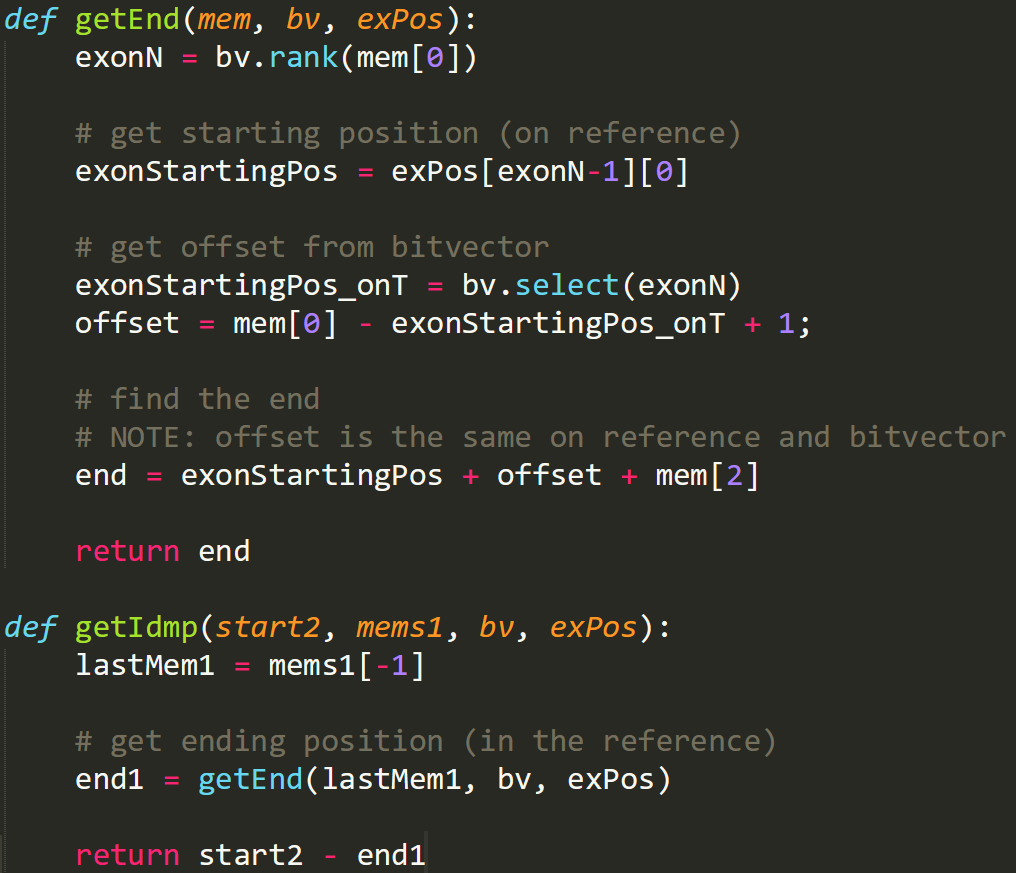
\includegraphics[width=\linewidth, height=9.5cm]{images/getIDMP.png}
%  \label{fig:GetIDMP}
%\end{figure}

\newpage

\subsection{TIDMP (Transcript-based IDMP)}
Per TIDMP si intende la misura della distanza \textit{sui trascritti} tra le due read. Per calcolarlo è innanzitutto necessario ottenere l'ultimo MEM relativo alla prima read e il primo MEM relativo alla seconda. Da ciascuno di essi è possibile ottenere la posizione iniziale e la lunghezza sul bitvector. 

A questo punto, usando l'operazione di rank, è possibile capire l'esone di provenienza di ciascun MEM.

Se i due MEM si trovano sullo stesso esone, il TIDMP è dato semplicemente dalla distanza tra la fine del primo MEM e l'inizio del secondo (sarà quindi uguale all' IDMP calcolato precedentemente).

Se i due MEM non si trovano sullo stesso esone, potrebbero essere su due esoni consecutivi o meno. Nel caso di esoni consecutivi, il TIDMP è dato dalla somma tra il suffisso non coperto dal primo esone e il prefisso non coperto dal secondo esone.

Il seguente frammento di codice mostra come calcolare il TIDMP:

\begin{lstlisting}[language=Python]
def getTranscriptIdmp(transcripts, mems1, mems2, bv, exPos):
    tIdmp = 0

    # get last mem from read1 and first mem from read2
    m1 = mems1[-1]
    m2 = mems2[0]

    # find exon for m1 and m2
    id1 = bv.rank(m1[0]) - 1
    id2 = bv.rank(m2[0]) - 1

    # find positions on bitvector
    start1 = m1[0]
    start2 = m2[0]
    len1 = m1[2]
    len2 = m2[2]

    if id1 == id2: # m1 and m2 are on same exon
        distance = start2 - (start1 + len1)
        tIdmp += distance
        
    else: # m1 and m2 are not on same exon
        consecutiveExons = False

        # check in all transcripts if the exons are consecutive
        # NOTE: two exons are consecutive if they appear 
        # next to each other in a transcript
        # (an exon is represented as (startPosReference, endPosReference))
        for _,exons in transcripts.items():
            start1Reference = getStart(m1,bv,exPos)
            start2Reference = getStart(m2,bv,exPos)
            end1Reference = getEnd(m1,bv,exPos)
            end2Reference = getEnd(m2,bv,exPos)
            for (s1, e1), (s2, e2) in pairwise(exons):
                if s1 == start1Reference and e1 == end1Reference
                    and s2 == start2Reference and e2 == end2Reference:
                    consecutiveExons = True
                    exon1EndingPosBv = bv.select(id1+1)
                    exon2startingPosBv = bv.select(id2)
                    distance = exon1EndingPosBv - (start1 + len1) 
                               + (start2 - exon2startingPosBv) - 1
                    tIdmp += distance
                    break

        if not consecutiveExons:
            pass

    return tIdmp
\end{lstlisting}

Il caso di esoni non consecutivi presenta diverse criticità, e per il momento non è stato calcolato.

\newpage

\section{Sviluppi futuri}

\subsection{Incremento della qualità degli allineamenti usando IDMP e TIDMP}

Innanzitutto, è fondamentale ricordare che la distanza tra le due read di un pair viene fornita dall'ente che ha effettuato il sequenziamento, ed è la stessa per tutta la libreria. Qualora non fosse disponibile, è possibile calcolarla effettuando un allineamento con allineatori come BWA\cite{li2013aligning} o STAR\cite{dobin2013star}, e lanciando un analisi sul BAM ottenuto con SAMTools (ovviamente lo stesso risultato si otterrebbe usando ASGAL come allineatore, ma non avrebbe senso usarlo come parametro).

Questo valore potrebbe essere usato come riferimento per effettuare gli allineamenti in ASGAL. Quando un allineamento ha un IDMP (calcolato da ASGAL) troppo diverso da quello fornito in input, l'allineamento potrebbe essere scartato. Un'altra possibilità potrebbe essere quella di provare a ri-allineare cercando un IDMP più basso. 

Un'altra possibilità potrebbe essere quella di utilizzare l'IDMP in fase di rilevazione, e attribuire un peso maggiore agli introni indotti da allineamenti (e quindi MEM) con un IDMP più simile a quello dato in input. Resta da formalizzare in che modo attribuire i pesi; questo approccio potrebbe inoltre avere conseguenze negative nella rilevazione di certi tipi di eventi.

Questi approcci hanno due problemi:
\begin{itemize}
	\item Non sempre la distanza viene fornita
	\item Non tutti gli allineatori hanno la stessa nozione di "distanza tra read" (ad esempio alcuni considerano anche tutta la prima read e tutta la seconda nel conteggio) e, visto che utilizzano politiche di allineamento differenti, i valori ottenuti possono differire.
\end{itemize}

Per provare a risolvere questi problemi, abbiamo provato ad introdurre il TIDMP, una statistica calcolata ad-hoc da ASGAL. Come detto sopra, per il momento viene calcolata solo nel caso di esoni consecutivi, andando quindi a perdere informazioni negli altri casi. Inoltre, non siamo ancora sicuri dell'effettiva utilità della stessa. Questo aspetto dovrà essere approfondito in futuro.

\newpage
    	
    	\section{Esempio di funzionamento}

In questo esempio di funzionamento si utilizzerà il gene ENSG00000280145, situato sul cromosoma 21 dell' uomo (Homo Sapiens, release GRCh38/hg38). E' stato prima scaricato il genoma di riferimento da ensembl\footnote{\url{https://www.ensembl.org/index.html}} in formato fasta e la relativa annotazione in formato gtf. Dal file gtf (contenente l'annotazione per l'intero genoma) è stata isolata l'annotazione relativa al gene ENSG00000280145.

\subsection{Generazione delle read con Flux Simuator}

Si è scelto di utilizzare Flux Simulator \cite{griebel2012modelling} per la generazione delle read paired-end. Il suo utilizzo non è particolarmente complicato, ma è necessario passare i diversi parametri attraverso un file con estensione .p. Il file utilizzato in questa simulazione è il seguente:

%\begin{figure}[thp]
%\begin{CenteredBox}
%  \begin{lstlisting}
%## File locations
%REF_FILE_NAME   annotation.gtf
%GEN_DIR         gen
%
%## Sequencing
%READ_NUMBER 2000
%READ_LENGTH 100
%PAIRED_END  YES
%FASTA   yes
%UNIQUE_IDS  YES
%
%POLYA_SCALE     NaN
%POLYA_SHAPE     NaN
%  \end{lstlisting}
%\end{CenteredBox}
%\caption{Il file contente i parametri di Flux Simulator}
%\end{figure}

\begin{figure}[h]
	\centering
	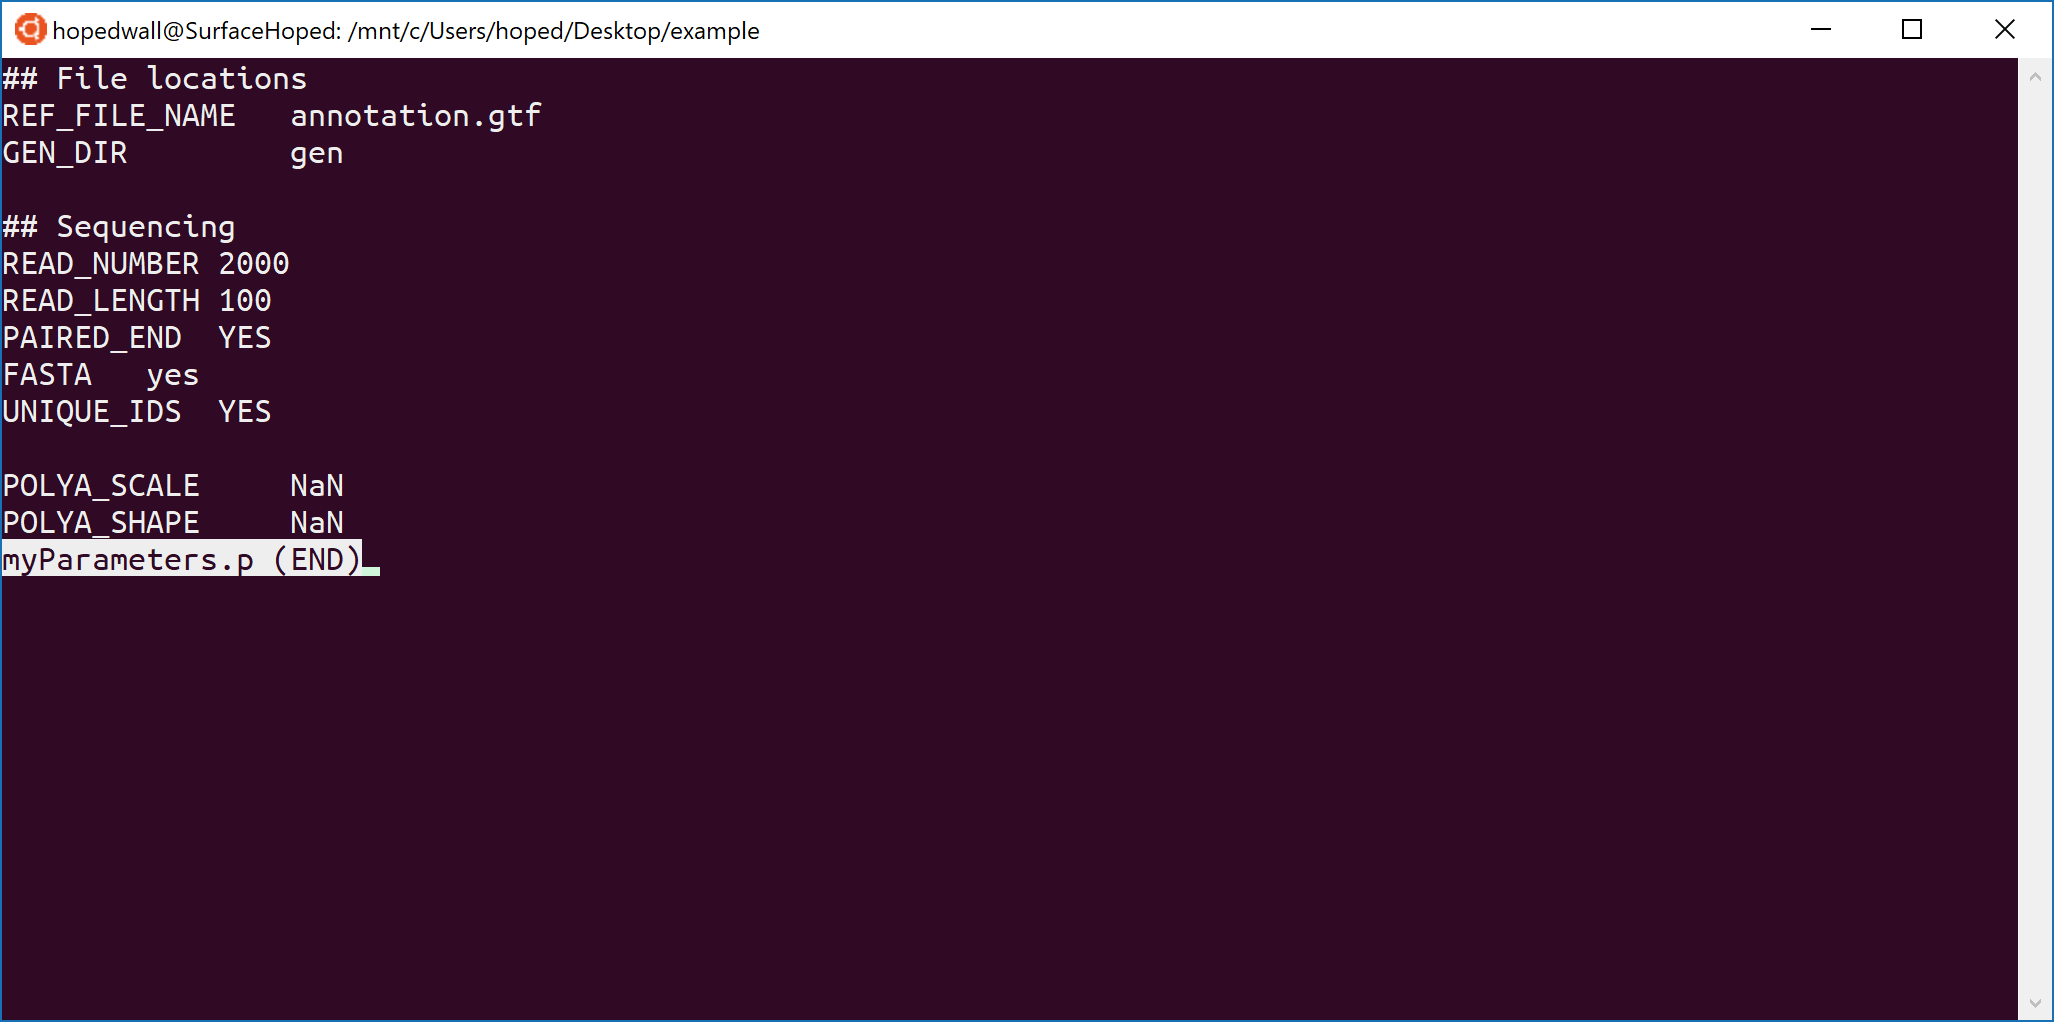
\includegraphics[width=\linewidth]{images/myParameters.png}
  \caption{Il file contente i parametri di Flux Simulator}
  \label{fig:Parameters}
\end{figure}

Vengono così generati due file contenti 2000 read di lunghezza 100, in formato fasta, che saranno dati in input ad ASGAL.

\newpage

\subsection{Utilizzo di ASGAL}

ASGAL viene eseguito via linea di comando, richiamando lo script principale usando come parametri:

\begin{itemize}
	\item Il \textbf{genoma} di riferimento (opzione \textbf{-g})
	\item L'\textbf{annotazione} del genoma (opzione \textbf{-a})
	\item I due file contenti \textbf{read} (opzioni \textbf{-s} e \textbf{-s2})
	\item La \textbf{cartella di destinazione} dell'output (opzione \textbf{-o})
	\item L'indicazione delle \textbf{read paired-end} (opzione \textbf{--paired})
	\item La \textbf{fragment library type} (opzione \textbf{-f}), opzionale per velocizzare la fase di allineamento
\end{itemize}

Questo script richiama nell'ordine lo Splice-Aware Aligner, il Formattatore SAM e il Rilevatore di eventi di Alternative Splicing, visualizzando alcune informazioni sul funzionamento.

Questa immagine mostra il funzionamento di ASGAL:

\begin{figure}[h]
	\centering
	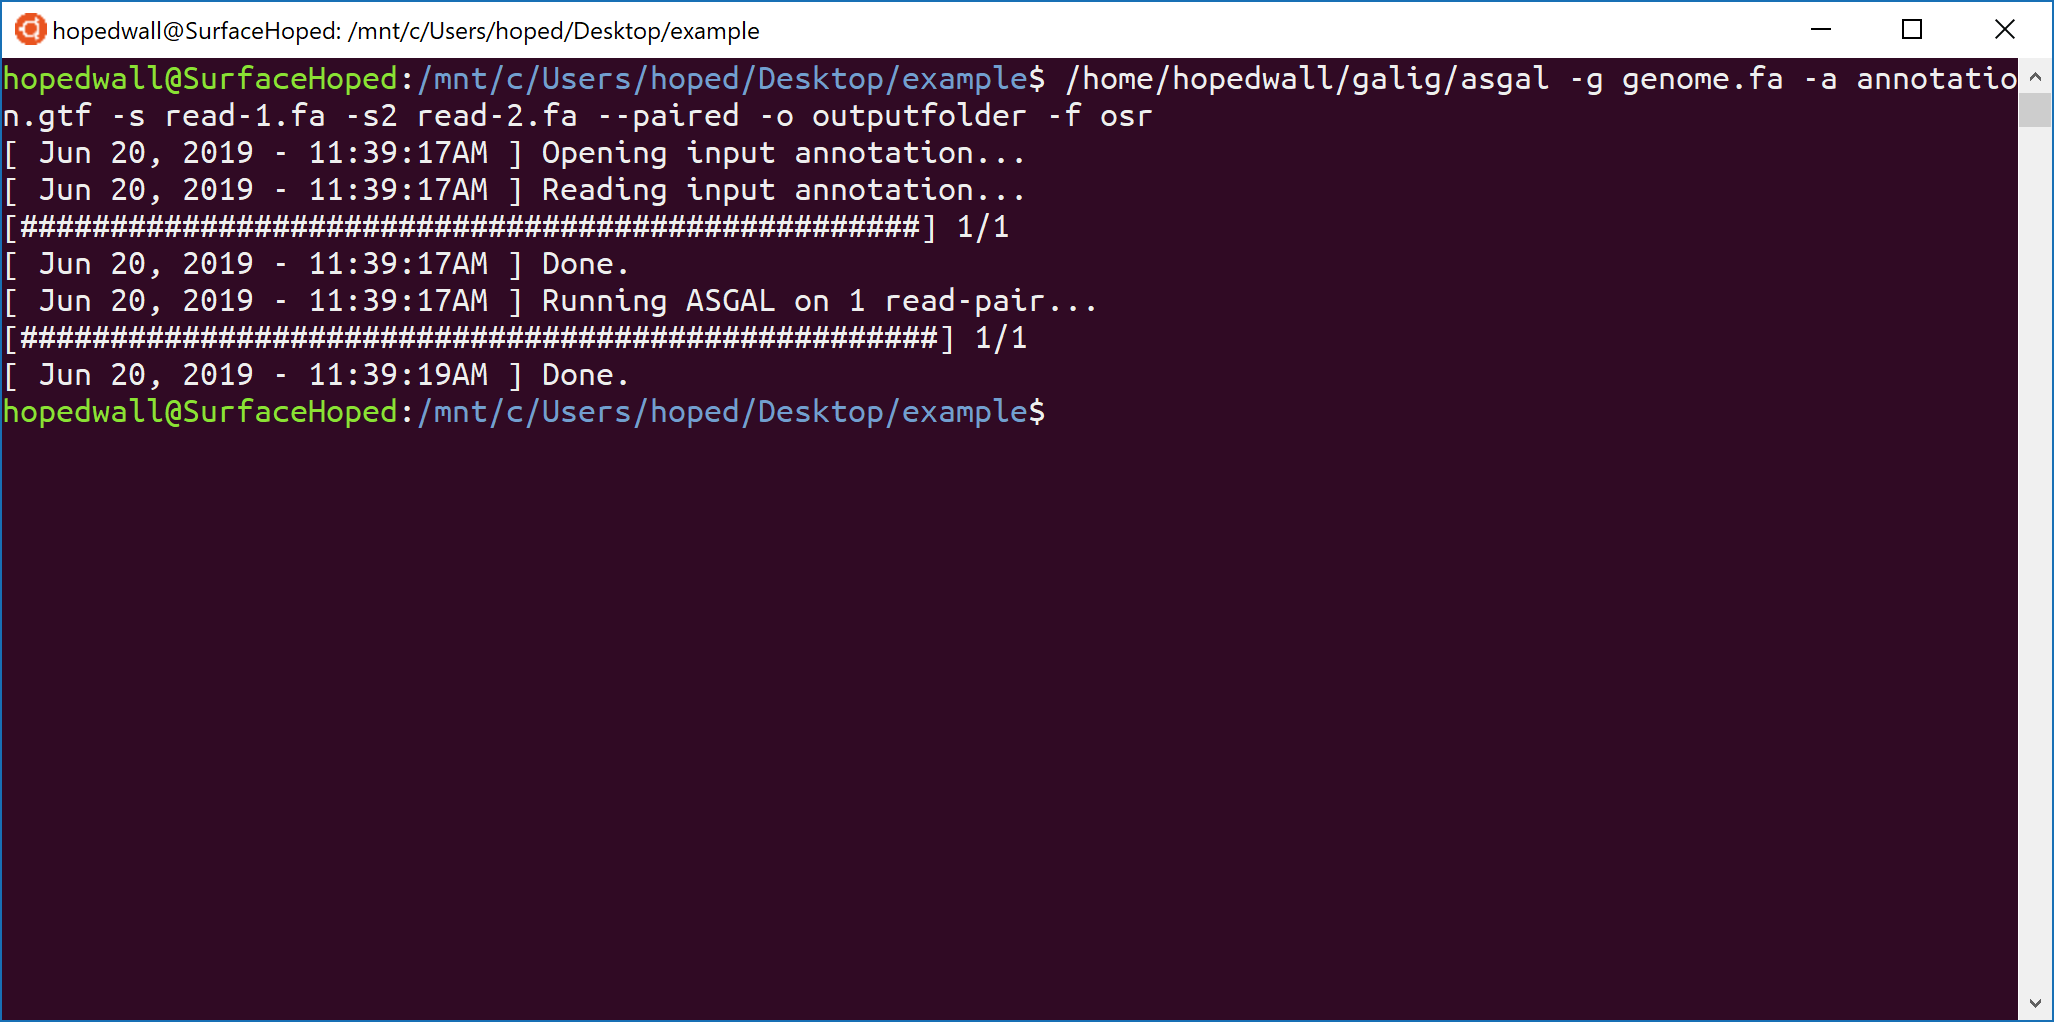
\includegraphics[width=\linewidth]{images/prompt.png}
  \caption{ASGAL in funzione}
  \label{fig:ASGALPrompt}
\end{figure}

Sebbene sia possibile eseguire ciascuno script singolarmente, si raccomanda di usare lo script principale per un utilizzo più immediato. 

\newpage

\subsection{Risultati}

Dall'esecuzione vengono prodotti i seguenti file:

\begin{figure}[h!]
	\centering
	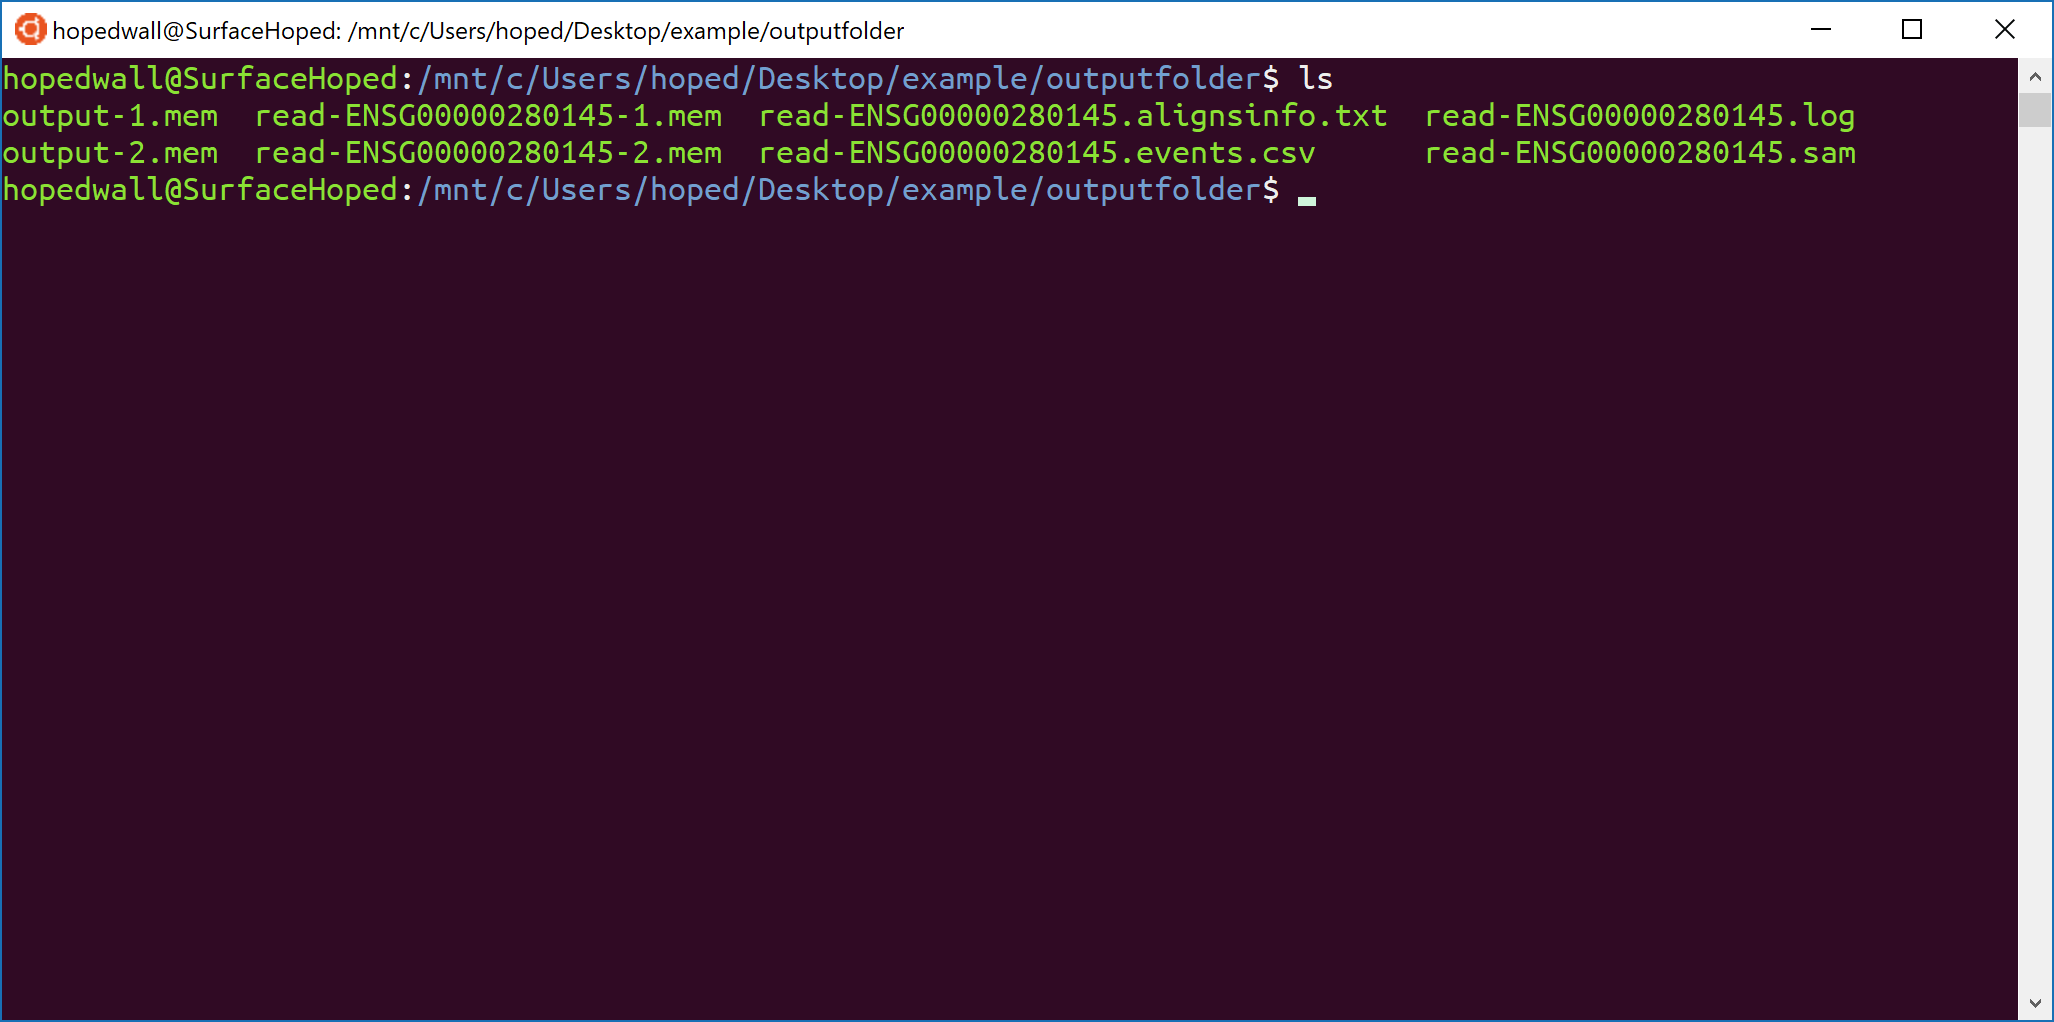
\includegraphics[width=\linewidth,height=10cm]{images/fileprodotti.png}
  \label{fig:ProducedFiles}
\end{figure}

Ovvero:

\begin{itemize}
	\item I file .mem prodotti dal primo step
	\item Il file .sam e .alignsinfo.txt prodotti dal secondo step
	\item	Il file .events.csv prodotti prodotto dal terzo step
\end{itemize}

%Utilizzando i seguenti comandi, è possibile preparare il file SAM per l'utilizzo con IGV (viene inoltre effettuato un controllo di correttezza del file SAM):
%
%\begin{figure}[h!]
%	\centering
%	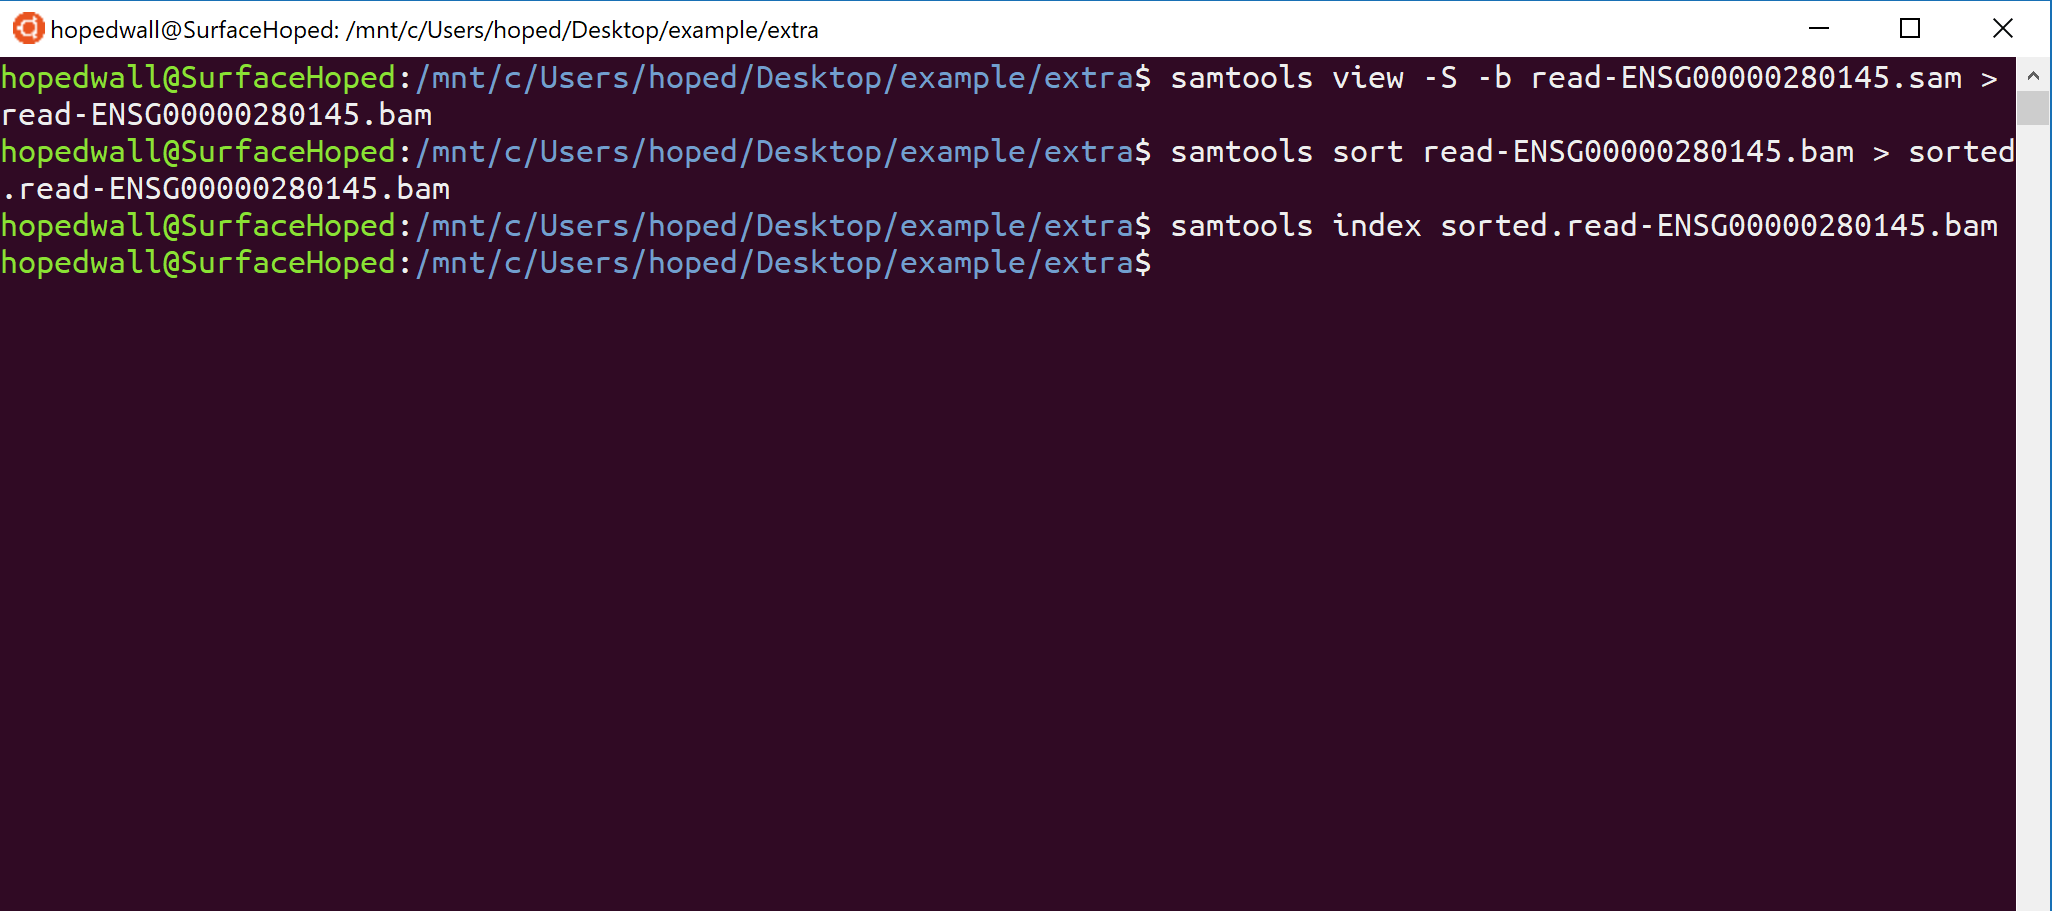
\includegraphics[width=\linewidth,height=10cm]{images/samtools.png}
%  \label{fig:SAMTools}
%\end{figure}
%
%\newpage

Analizzando il file alignsinfo.txt si nota che oltre il 98\% delle read sono state mappate.

\begin{figure}[h!]
	\centering
	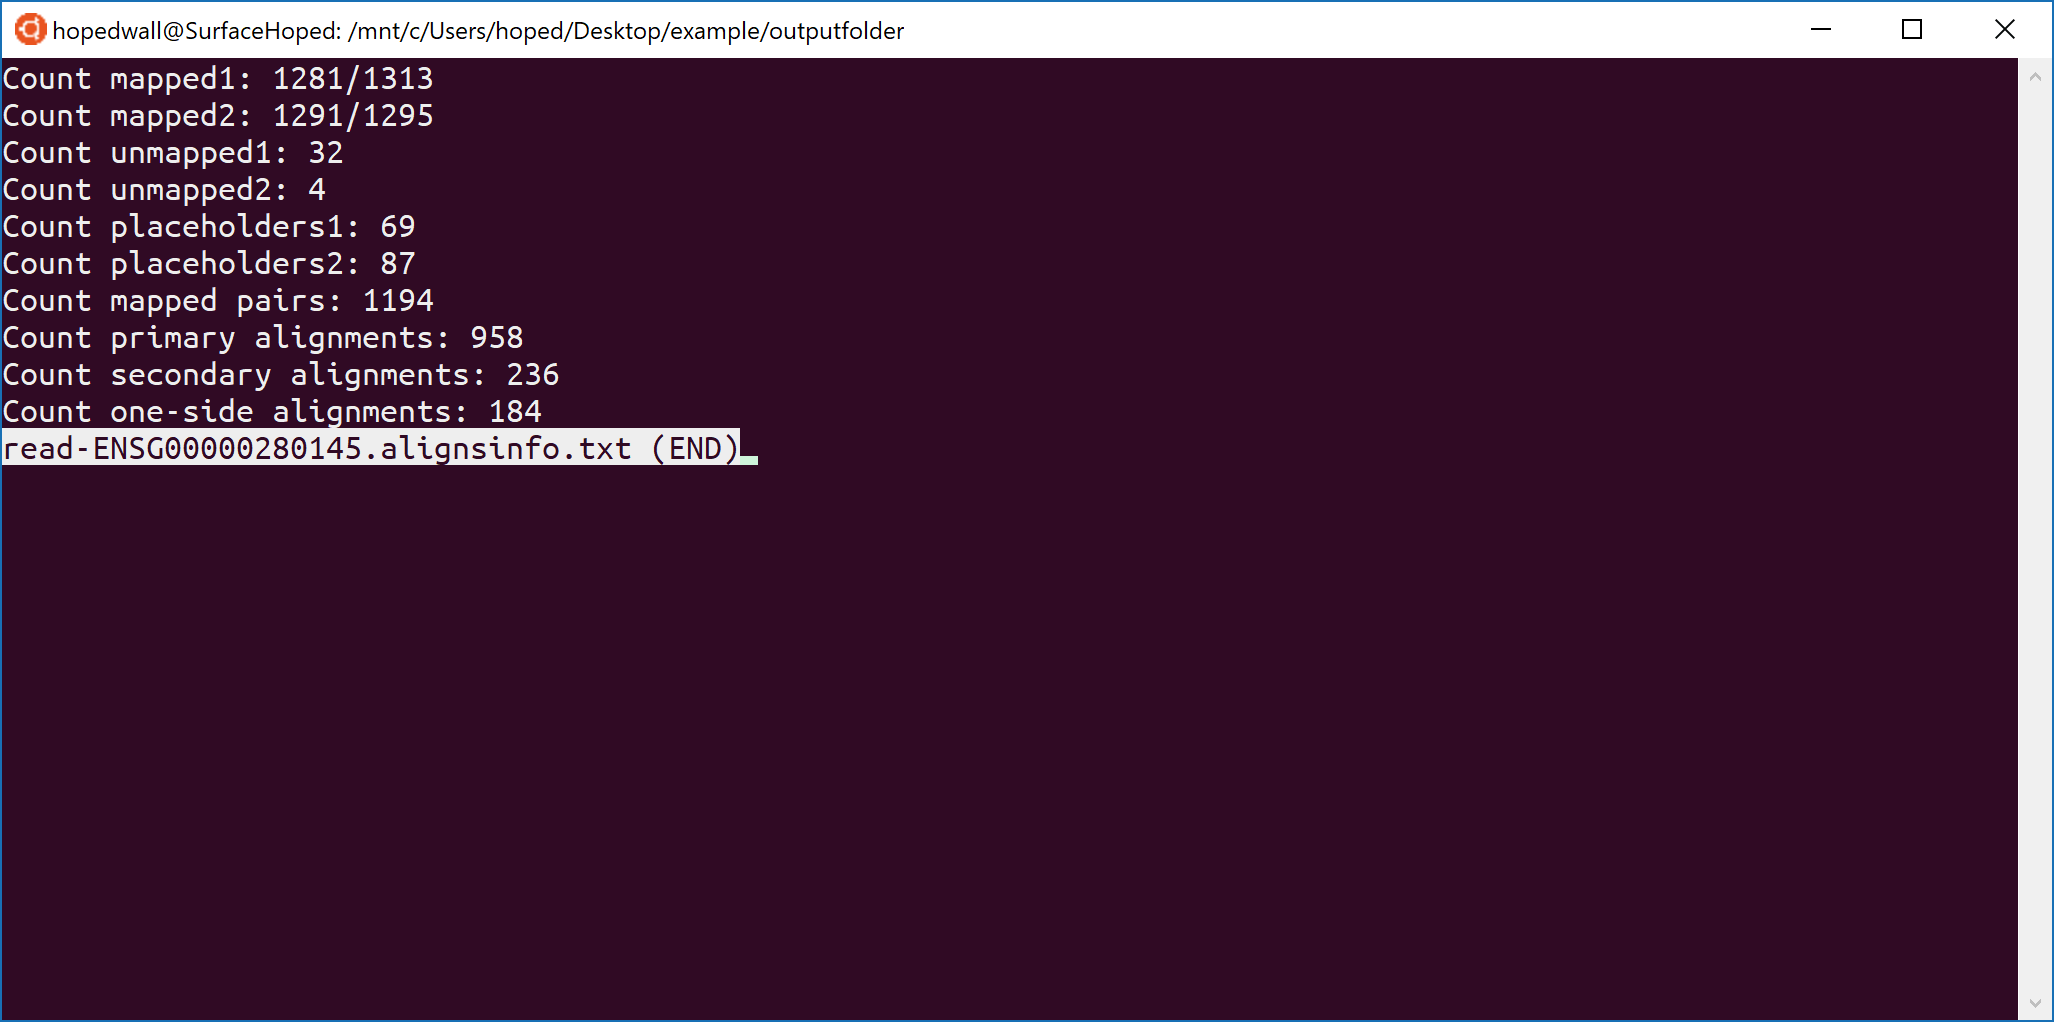
\includegraphics[width=\linewidth,height=10cm]{images/alignsinfotxt.png}
  \label{fig:AlignsInfoExperiment}
\end{figure}

\newpage

Il file events.csv contiene gli eventi di Alternative Splicing rilevati da ASGAL:

%\begin{itemize}
%	\item la prima colonna rappresenta il \textbf{tipo di evento}
%	\item la seconda colonna rappresenta la \textbf{posizione di inizio} nella genomica
%	\item	la terza colonna rappresenta la \textbf{posizione di fine} nella genomica
%	\item la quarta colonna rappresenta il \textbf{numero di read} che suggeriscono l'evento
%	\item la quinta colonna rappresenta il/i \textbf{nomi dei trascritti} che suggeriscono l'evento
%\end{itemize}

\begin{figure}[h!]
	\centering
	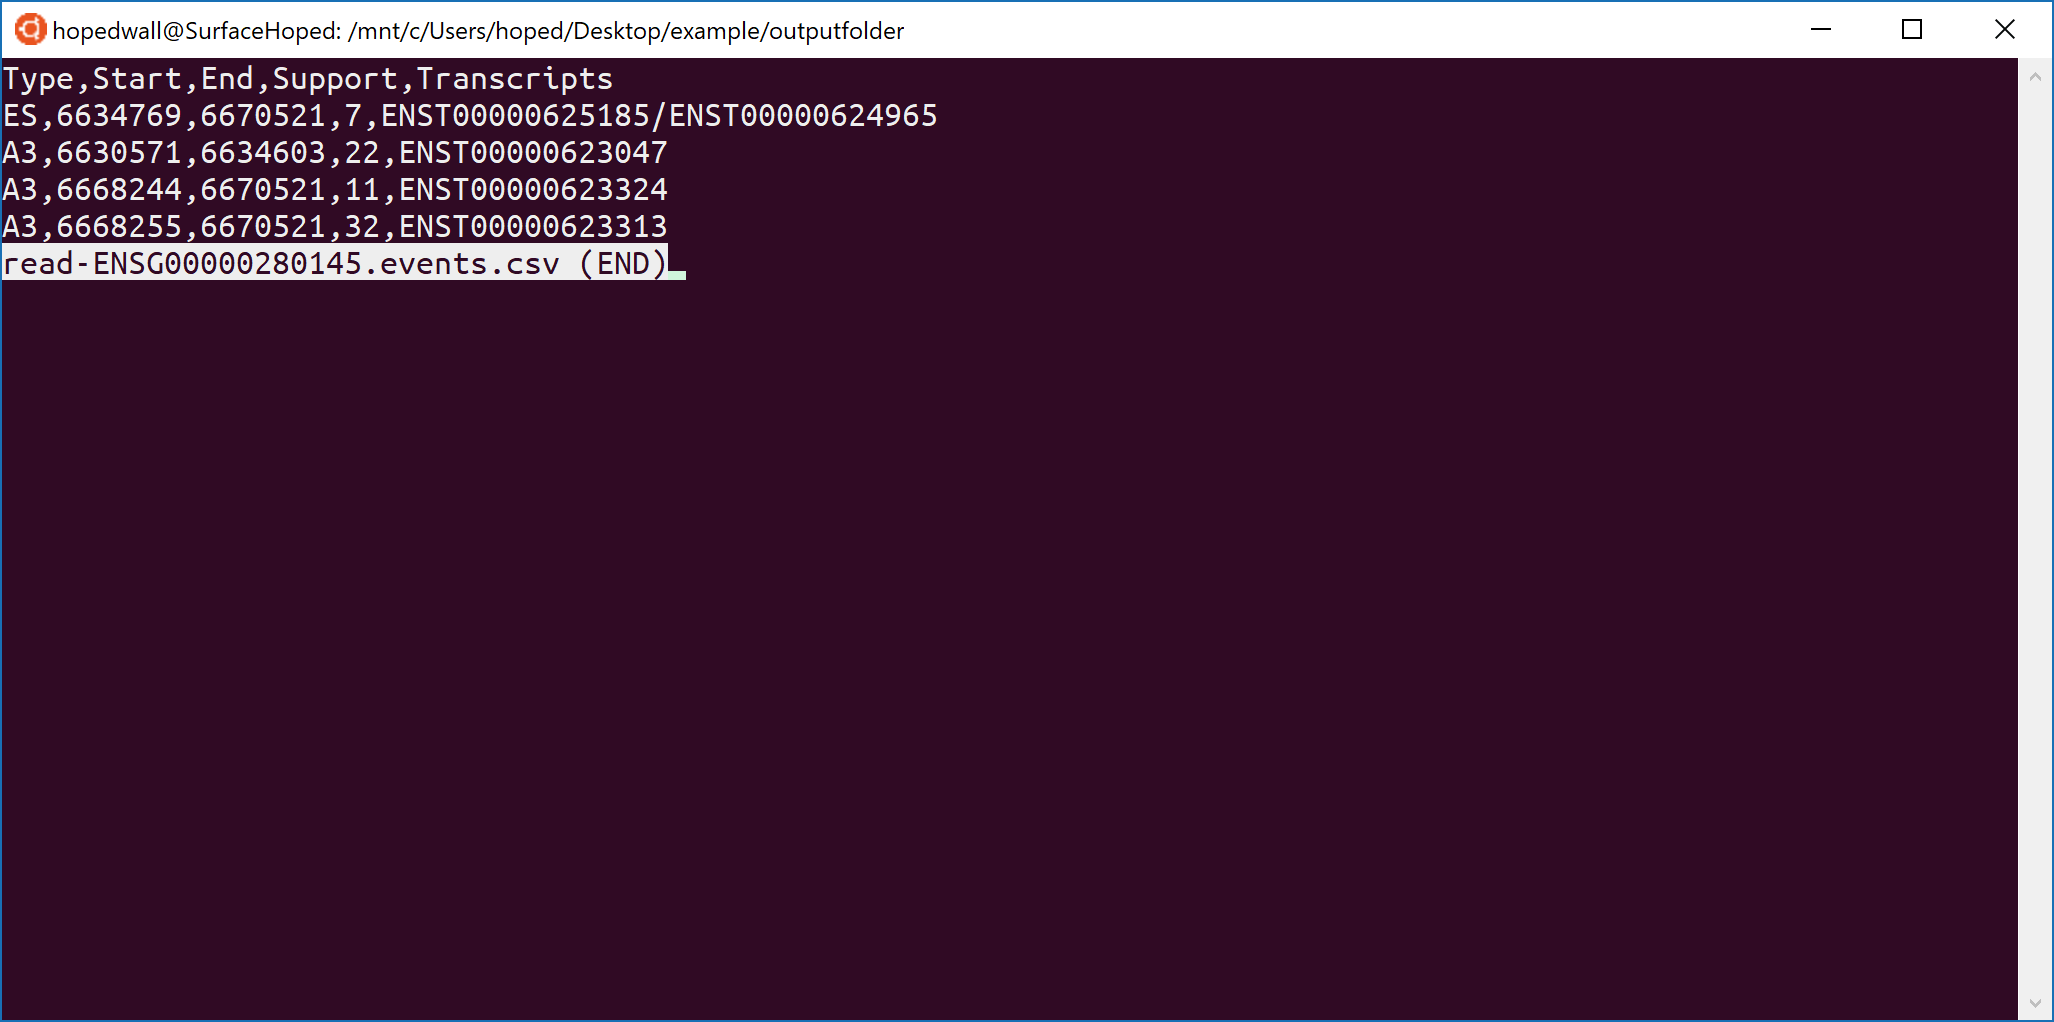
\includegraphics[width=\linewidth]{images/results.png}
  \label{fig:Parameters}
\end{figure}

Sono stati rilevati tre eventi di Alternative Donor Site e un evento di Exon Skipping.

\newpage
    	
    	\section{Competenze acquisite durante lo svolgimento dello stage}
    	
		\section{Conclusioni}
		
		\begin{thebibliography}{9}

			\bibitem{ASGAL}
			Denti L, Rizzi R, Beretta S, Vedova GD, Previtali M, Bonizzoni P. ASGAL: aligning RNA-Seq data to a splicing graph to detect novel alternative splicing events. BMC Bioinformatics. 2018;19(1):444. Published 2018 Nov 20. doi:10.1186/s12859-018-2436-3
			
			\bibitem{MEM}
 Beretta S, Bonizzoni P, Denti L, Previtali M, Rizzi R.Mapping rna-seq data to a transcript graph via approximate pattern matching to a hypertext. In: International Conference on Algorithms for Computational Biology. Berlin:Springer;2017. p.49–61. 
			
			\bibitem{ASExon}
				Wang ET,  Sandberg R,  Luo S,  Khrebtukova I,  Zhang L,  Mayr C,  Kingsmore SF,  Schroth GP,  Burge CB. Alternative isoform regulation in human tissue transcriptomes, Nature , 2008, vol. 462 (pg. 470-476)
				
			\bibitem{ASDiseases}
Tazi J, Bakkour N, Stamm S. Alternative splicing and disease. Biochim Biophys Acta. 2009;1792(1):14–26. doi:10.1016/j.bbadis.2008.09.017
							
			\bibitem{ASAlzheimer}
			Love JE, Hayden EJ, Rohn TT. Alternative Splicing in Alzheimer's Disease. J Parkinsons Dis Alzheimers Dis. 2015;2(2):6. doi:10.13188/2376-922X.1000010
			
			\bibitem{FLT}
			Salmon Documentation, Rob Patro, Geet Duggal, Mike Love, Rafael Irizarry and Carl Kingsford. Can be found at: \textit{https://salmon.readthedocs.io/en/latest/}
			
			\bibitem{SAM}
			Sequence Alignment/Map Format Specification, The SAM/BAM Format Specification Working Group, 14 May 2019. Can be found at: \textit{http://samtools.github.io/hts-specs/SAMv1.pdf}
			
			\bibitem{IGV}
			Thorvaldsdóttir H, Robinson JT, Mesirov JP. Integrative Genomics Viewer (IGV): high-performance genomics data visualization and exploration. Brief Bioinform. 2013;14(2):178–192. doi:10.1093/bib/bbs017
			
		\end{thebibliography}

\end{document}
